\documentclass[a4paper]{article}

\def\ssver{4.0.05}

\usepackage[left=1cm,right=1cm,top=0.75cm,bottom=2cm]{geometry}
\usepackage{xcolor}
\usepackage{pdfpages}
\usepackage{fancyhdr}
\usepackage{hyperref}
\usepackage{makeidx}
\usepackage{graphicx}
\usepackage{adjustbox}
\usepackage{multicol}
\usepackage{totcount}
\usepackage{xcolor}

% Default settings
\def\musicmode{0}
\def\largeprintmode{0}

% Large print sizes
\if\largeprintmode 1%
  \renewcommand{\tiny}{\fontsize{17}{22.5}\selectfont}%
  \renewcommand{\scriptsize}{\fontsize{19}{25.5}\selectfont}%
  \renewcommand{\footnotesize}{\fontsize{21}{28.5}\selectfont}%
  \renewcommand{\small}{\fontsize{23}{31.5}\selectfont}%
  \renewcommand{\normalsize}{\fontsize{24}{33}\selectfont}%
  \renewcommand{\large}{\fontsize{26}{36}\selectfont}%
  \renewcommand{\Large}{\fontsize{28}{39}\selectfont}%
  \renewcommand{\LARGE}{\fontsize{31}{43.5}\selectfont}%
  \renewcommand{\huge}{\fontsize{34}{48}\selectfont}%
  \renewcommand{\Huge}{\fontsize{38}{54}\selectfont}%
\fi

% Index
\if\largeprintmode 1%
  \usepackage[columns=1]{idxlayout}%
\fi
\makeindex

% Counters
\newtotcounter{songcount}
\newtotcounter{psalmcount}
\definecolor{title dark}{HTML}{7E73A7}

% Footer
\pagestyle{fancy}
\fancyhf{}
\cfoot{{\small\thepage}\if\largeprintmode 1\else \\ {\footnotesize Corrections and additions email: songsheet@daniellaing.com{\quad}v{\ssver}}\fi}
\renewcommand{\headrulewidth}{0pt}

\makeatletter

% Chorus
\newcommand{\chorus}{\@chorusi}
\newcommand{\@chorusi}{\@ifnextchar\end{\@chorusend}{\@chorusii}}
\newcommand{\@chorusii}[1]{\quad{\itshape#1}\par\@chorusi}
\newcommand{\@chorusend}[1]{\vskip1em}

% --------------------

% Verse
\renewcommand{\verse}{\@versei}
\newcommand{\@versei}{\@ifnextchar\end{\@verseend}{\@verseii}}
\newcommand{\@verseii}[1]{#1\par\@versei}
\newcommand{\@verseend}[1]{\vskip1em}

% --------------------

% Bridge
\newcommand{\bridge}{\@bridgei}
\newcommand{\@bridgei}{\@ifnextchar\end{\@bridgeend}{\@bridgeii}}
\newcommand{\@bridgeii}[1]{{\itshape#1}\par\@bridgei}
\newcommand{\@bridgeend}[1]{\vskip1em}

\makeatother

\newenvironment{song}[1]{\if\largeprintmode 1\else\begin{minipage}[t]{0.94\columnwidth}\fi{\stepcounter{songcount}\textbf{\large #1}\index{#1}}\par\vskip2pt}{\if\largeprintmode 1\pagebreak\else\end{minipage}\fi\vskip2em}
\newenvironment{psalm}[2]{\if\largeprintmode 1\else\begin{minipage}[t]{0.94\columnwidth}\fi\begin{center}{\stepcounter{psalmcount}\textbf{\large #1}\index{#1}  {\normalsize #2}}\par\vskip2pt}{\end{center}\if\largeprintmode 1\pagebreak\else\end{minipage}\fi\vskip2em}

\newcommand{\extra}[1]{{\normalsize\itshape (#1)}}

\renewcommand{\sp}{{\normalsize\itshape (Sing Psalms)}}
\newcommand{\tr}{{\normalsize\itshape (Scottish Psalter)}}
\newcommand{\LORD}{{\scshape Lord}}

% Chords
\definecolor{chordColor}{HTML}{CC241D}
\newcommand{\m}[2][l]%
{%
  \if\musicmode 1%
    \makebox[0pt][#1]%
    {%
      \begin{tabular}[b]%
        {@{}l@{}}%
        {\normalsize\mdseries\color{chordColor}#2}%
        \\%
        \mbox{}%
      \end{tabular}%
    }%
  \fi%
}
\newcommand{\mm}[1]{\if\musicmode 1 #1 \fi}


% Settings

\def\musicmode{0}


\begin{document}
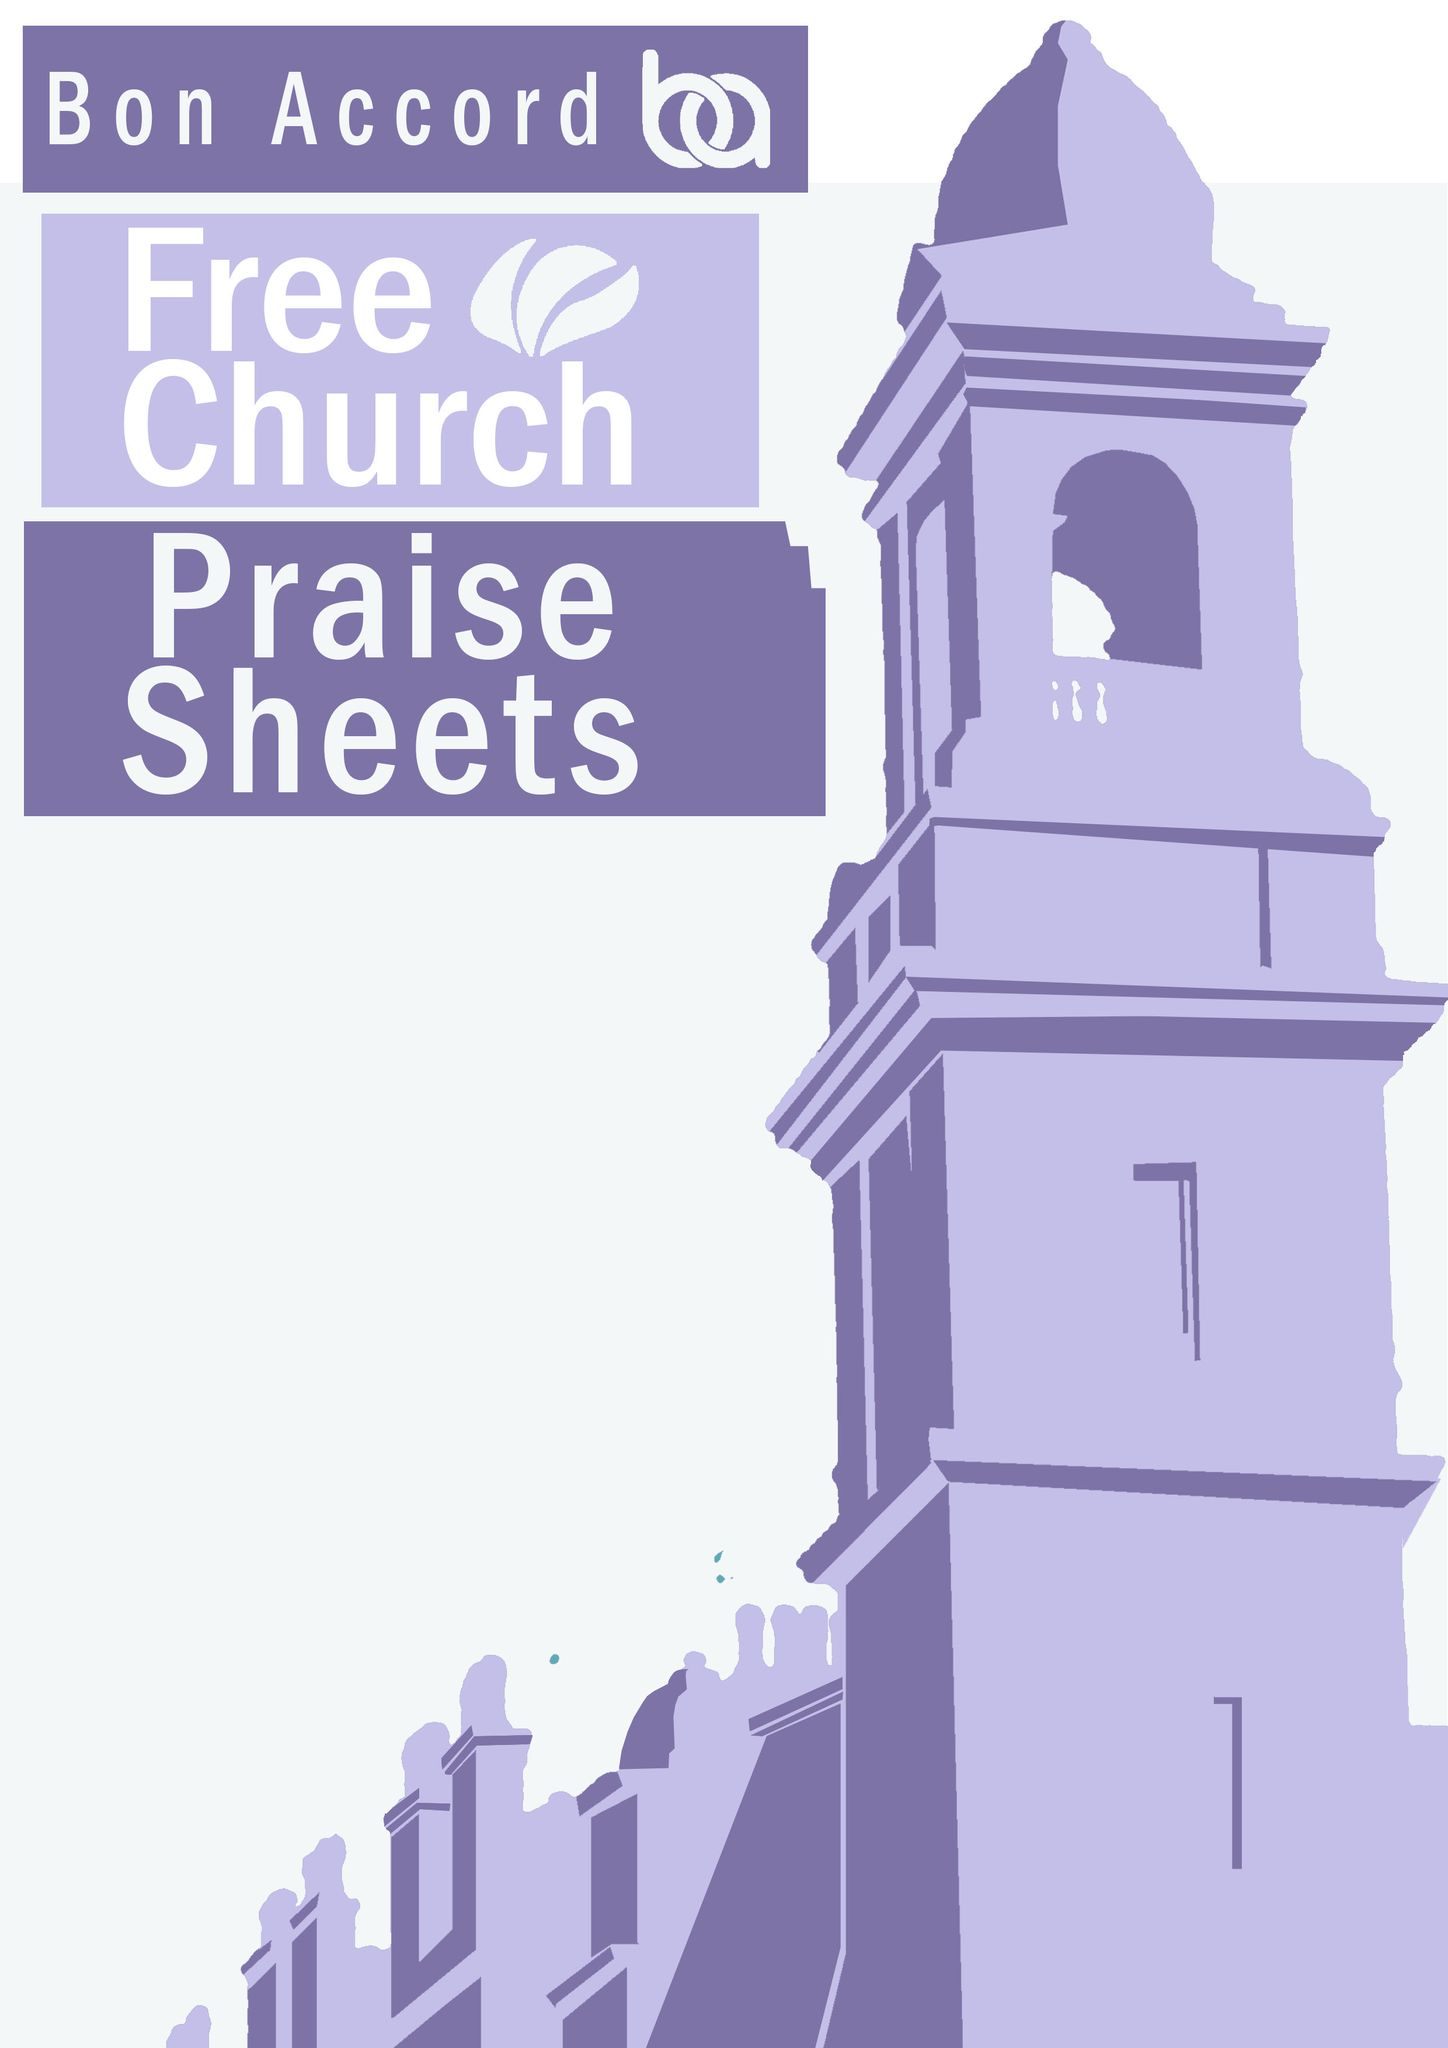
\includepdf{titleimage.jpg}
\setcounter{page}{2}  % Make title page, page 1
\printindex
\if\largeprintmode 1\pagebreak\fi

% --------------------
\if\largeprintmode 1\else
  \begin{multicols}{2}
  \raggedcolumns
\fi

\begin{song}{5 Hymn Medley}
    \verse
    {O, when the saints go marching in,}
    {O, when the saints go marching in,}
    {How I want to b in that number,}
    {When the saints go marching in.}
    \end
    \verse
    {I'm gonna sing, sing, sing,}
    {I'm gonna shout, shout, shout,}
    {I'm gonna sing, I'm gonna shout, praise the Lord!}
    {When those gates are open wide,}
    {I'm gonna sit at Jesus' side,}
    {I'm gonna sing, I'm gonna shout, praise the Lord!}
    \end
    \verse
    {O the land of the cloudless day,}
    {O the land of home,}
    {O the land where no storm clouds rise,}
    {O the land of cloudless day.}
    \end
    \verse
    {Swing low, sweet chariot,}
    {Coming fro to carry me home,}
    {Swing low, sweet chariot,}
    {Coming fro to carry me home.}
    \end
    \verse
    {This train is bound for glory, this train,}
    {This train is bound for glory, this train,}
    {This train is bound for glory, O what a wonderous story,}
    {This train is bound for glory, this train.}
    \end
\end{song}

% ---

\begin{song}{Abide With Me}
    \verse
    {Abide with me; fast falls the eventide;}
    {The darkness deepens; Lord, with me abide;}
    {When other helpers fail and comforts flee,}
    {Help of the helpless, O abide with me.}
    \end
    \verse
    {Swift to its close ebbs out life's little day;}
    {Earth's joys grow dim, its glories pass away;}
    {Change and decay in all around I see-}
    {O Thou who changest not, abide with me.}
    \end
    \verse
    {I need Thy presence every passing hour;}
    {What but Thy grace can foil the tempter's pow'r?}
    {Who, like Thyself, my guide and stay can be?}
    {Through cloud and sunshine, Lord, abide with me.}
    \end
    \verse
    {I fear no foe, with Thee at hand to bless;}
    {Ills have no weight, and tears no bitterness;}
    {Where is death's sting? Where, grave, thy victory?}
    {I triumph still, if Thou abides with me.}
    \end
    \verse
    {Hold Thou Thy cross before my closing eyes;}
    {Shine through the gloom and point me to the skies;}
    {Heav'n's morning breaks, and Earth's vain shadows flee;}
    {In life, in death, O Lord, abide with me.}
    \end
\end{song}

% ---

\begin{song}{Across The Lands}
    \verse
    {You're the \m{C}Word of \m{G}God the \m{F}Father,}
    {From be\m{C}fore the \m{G}world began;}
    {Every \m{F}star and every \m{C}planet}
    {Has been \m{Dm}fashioned by Your \m{F}hand.}
    {All cre\m{C}ation \m{G}holds to\m{F}gether}
    {By the \m{C}power \m{G}of Your voice}
    {Let the \m{F}skies declare Your \m{C}glory}
    {Let the \m{Dm}land and \m{F}seas re\m{G}joice!}
    \end
    \chorus
    {You're the \m{F}Author of cre\m{C}ation,}
    {You're the \m{F}Lord of \m{G}every \m{Am}man;}
    {And Your \m{F}cry of love rings \m{Am}out}
    {A\m{G}cross the \m{C}lands.}
    \end
    \verse
    {Yet You left the gaze of angels,}
    {Came to seek and save the lost,}
    {And exchanged the joy of Heaven}
    {For the anguish of a cross.}
    {With a prayer you fed the hungry,}
    {With a word You stilled the sea.}
    {Yet how silently You suffered}
    {That the guilty may go free.}
    \end
    \verse
    {With a shout You rose victorious,}
    {Wrestling victory from the grave,}
    {And ascended into Heaven}
    {Leading captives in Your wake.}
    {Now You stand before the Father}
    {Interceding for Your own;}
    {From each tribe and tongue and nation,}
    {You are leading sinners home!}
    \end
\end{song}

% ---

\begin{song}{All Creatures Of Our God And King}
    \verse
    {All Creatures Of Our God And King}
    {Lift up your voice and with us sing,}
    {O praise Him! Alleluia!}
    {Thou burning sun with golden beam,}
    {Thou silver moon with softer gleam!}
    {{\itshape O praise Him! O praise Him!}}
    {{\itshape Alleluia! Alleluia! Alleluia!}}
    \end
    \verse
    {All Creatures Of Our God And King}
    {Lift up your voice and with us sing,}
    {O praise Him! Alleluia!}
    {Thou burning sun with golden beam,}
    {Thou silver moon with softer gleam!}
    {{\itshape O praise Him! O praise Him!}}
    {{\itshape Alleluia! Alleluia! Alleluia!}}
    \end
    \verse
    {All Creatures Of Our God And King}
    {Lift up your voice and with us sing,}
    {O praise Him! Alleluia!}
    {Thou burning sun with golden beam,}
    {Thou silver moon with softer gleam!}
    {{\itshape O praise Him! O praise Him!}}
    {{\itshape Alleluia! Alleluia! Alleluia!}}
    \end
\end{song}

% ---

\begin{song}{All Glory Be To Christ}
    \verse
    {Should nothing of our efforts stand}
    {No legacy survive}
    {Unless the Lord does raise the house}
    {In vain its builders strive}
    {To you who boast tomorrow's gain}
    {Tell me, What is your life?}
    {A mist that vanishes at dawn}
    {All glory be to Christ!}
    \end
    \chorus
    {All glory be to Christ our king!}
    {All glory be to Christ!}
    {His rule and reign we'll ever sing}
    {All glory be to Christ!}
    \end
    \verse
    {His will be done, His kingdom come}
    {On Earth as is above}
    {Who is Himself our daily bread}
    {Praise Him, the Lord of love}
    {Let living water satisfy}
    {The thirsty without price}
    {We'll take a cup of kindness yet}
    {All glory be to Christ!}
    \end
    \verse
    {When on the day the great I Am}
    {The faithful and the true}
    {The Lamb who was for sinners slain}
    {Is making all things new}
    {Behold our God shall live with us}
    {And be our steadfast light}
    {And we shall e'er his people be}
    {All glory be to Christ!}
    \end
\end{song}

% ---

\begin{song}{All I Have Is Christ}
    \verse
    {I once was lost in darkest night}
    {Yet thought I knew the way}
    {The sin that promised joy and life}
    {Had led me to the grave}
    {I had no hope that You would own}
    {A rebel to Your will}
    {And if You had not loved me first}
    {I would refuse You still}
    \end
    \chorus
    {Hallelujah! All I have is Christ}
    {Hallelujah! Jesus is my life}
    \end
    \verse
    {But as I ran my hell-bound race}
    {Indifferent to the cost}
    {You looked upon my helpless state}
    {And led me to the cross}
    {And I beheld God's love displayed}
    {You suffered in my place}
    {You bore the wrath reserved for me}
    {Now all I know is grace}
    \end
    \verse
    {Now, Lord, I would be Yours alone}
    {And live so all might see}
    {The strength to follow Your commands}
    {Could never come from me}
    {O Father, use my ransomed life}
    {In any way You choose}
    {And let my song forever be}
    {My only boast is You}
    \end
\end{song}

% ---

\begin{song}{All I Once Held Dear \extra{Knowing You}}
    \verse
    {All I once held dear, built my life upon}
    {All this world reveres, and wars to own}
    {All I once thought gain I have counted loss}
    {Spent and worthless now, compared to this}
    \end
    \chorus
    {Knowing you, Jesus, knowing you,}
    {There is no greater thing}
    {You're my all, you're my best}
    {You're my joy, my righteousness}
    {And I love you, Lord}
    \end
    \verse
    {Now my heart's desire is to know you more}
    {To be found in you and known as yours}
    {To possess by faith what I could not earn}
    {All-surpassing gift of righteousness}
    \end
    \verse
    {Oh, to know the power of your risen life}
    {And to know You in Your sufferings}
    {To become like you in your death, my Lord}
    {So with you to live and never die}
    \end
\end{song}

% ---

\begin{song}{Amazing Grace \extra{My Chains Are Gone}}
    \verse
    {Amazing grace, how sweet the sound}
    {That saved a wretch like me}
    {I once was lost, but now I'm found}
    {Was blind, but now I see}
    \end
    \verse
    {`Twas grace that taught my heart to fear}
    {And grace my fears relieved}
    {How precious did that grace appear}
    {The hour I first believed}
    \end
    \chorus
    {My chains are gone}
    {I've been set free}
    {My God, my Saviour has ransomed me}
    {And like a flood His mercy reigns}
    {Unending love, amazing grace}
    \end
    \verse
    {The Lord has promised good to me}
    {His word my hope secures}
    {He will my shield and portion be}
    {As long as life endures.}
    \end
    \verse
    {The Earth shall soon dissolve like snow}
    {The sun forbear to shine}
    {But God, Who called me here below,}
    {Will be forever mine.}
    \end
\end{song}

% ---

\begin{song}{Amazing Grace}
    \verse
    {Amazing grace! How sweet the sound}
    {That saved a wretch like me!}
    {I once was lost but now am found;}
    {Was blind but now I see.}
    \end
    \verse
    {‘Twas grace that taught this heart to fear,}
    {And grace my fears relieved;}
    {How precious did that grace appear}
    {The hour I first believed.}
    \end
    \verse
    {Through many dangers toils and snares,}
    {I have already come;}
    {‘Tis grace that brought me safe thus far,}
    {And grace will lead me home.}
    \end
    \verse
    {The Lord has promised good to me,}
    {His Word my hope secures;}
    {He will my Shield and Portion be,}
    {As long as life endures.}
    \end
    \verse
    {When we've been there ten thousand years,}
    {Bright shining as the Sun;}
    {We've no less days to sing God's praise,}
    {Than when we've first begun.}
    \end
\end{song}

% ---

\begin{song}{And Can It Be}
    \verse
    {\m{G}And can it \m{Em}be that \m{C}I \m{D}should \m{G}gain}
    {An \m{C}in\m{D}t'rest \m{G}in the \m{D}Sav\m{A}iour's \m{D}blood?}
    {Died He for \m{G}me\m{D}, who \m{G}caused \m{Em}His \m{D}pain --}
    {For \m{C}me, who \m{G}Him to \m{Em}death \m{D}pur\m{G}sued?}
    {A\m{D}mazing \m{G}love! \m{Em}How \m{C}can\m{Am} it \m{D}be,}
    {That \m{G}Thou, my \m{C}God, shouldst \m{D}die for \m{G}me?}
    {\quad{\itshape Amazing \m{D}love! How \m{D7}can it \m{G}be,}}
    {\quad{\itshape That \m{C}Thou, my \m{G}God, \m{C}shouldst \m{G}die \m{D}for \m{G}me!}}
    \end
    \verse
    {'Tis mystery all: th'Immortal dies:}
    {Who can explore is strange design?}
    {In vain the firstborn seraph tries}
    {To sound the depths of love diving.}
    {‘Tis mercy all! Let Earth adore;}
    {Let angel minds enquire no more.}
    \end
    \verse
    {He left His Father's throne above}
    {So free, so infinite His grace-}
    {Emptied Himself of all but love,}
    {And bled for Adam's helpless race:}
    {‘Tis mercy all, immense and free,}
    {For, O my God it found out me!}
    \end
    \verse
    {No condemnation now I dread;}
    {Jesus, and all in Him, is mine;}
    {Alive in His, my living Head,}
    {And clothed in righteousness divine,}
    {Bold I approach th'eternal throne,}
    {And claim the crown, through Christ my own.}
    \end
\end{song}

% ---

\begin{song}{A Safe Stronghold}
    \verse
    {A safe stronghold our God is still,}
    {A trusty shield and weapon;}
    {He'll help us clear from all the ill}
    {That hath us now o'ertaken.}
    {The ancient prince of hell}
    {Hath risen with purpose fell;}
    {Strong mail of craft and power}
    {He weareth in this hour;}
    {On Earth is not his fellow.}
    \end
    \verse
    {With force of arms we nothing can,}
    {Full soon were we down-ridden;}
    {But for us fights the proper Man,}
    {Whom God Himself hath bidden.}
    {Ask ye, who is this same?}
    {Christ Jesus is His name,}
    {The Lord Sabaoth's Son;}
    {He, and no other one,}
    {Shall conquer in the battle.}
    \end
    \verse
    {And were this world all devils o'er,}
    {And watching to devour us,}
    {We lay it not to heart so sore;}
    {Not they can overpower us.}
    {And let the prince of ill}
    {Look grim as e'er he will,}
    {He harms us not a whit;}
    {For why? His doom is writ;}
    {A word shall quickly slay him.}
    \end
    \verse
    {God's Word, for all their craft and force,}
    {One moment will not linger,}
    {But, spite of hell, shall have its course;}
    {'Tis written by His finger.}
    {And though they take our life,}
    {Goods, honour, children, wife,}
    {Yet is their profit small;}
    {These things shall vanish all:}
    {The City of God remaineth!}
    \end
\end{song}

% ---

\begin{song}{As The Deer Pants}
    \verse
    {As the deer pants for the water}
    {So my soul longs after Thee.}
    {You alone are my heart's desire}
    {And I long to worship You}
    \end
    \chorus
    {You alone are my Strength, my Shield}
    {To You alone may my spirit yield}
    {You alone are my heart's desire}
    {And I long to worship Thee}
    \end
    \verse
    {You're my friend and You are my brother,}
    {Even though you are a king.}
    {I love You more than any other,}
    {So much more than anything.}
    \end
    \verse
    {I want You more than gold or silver,}
    {Only You can satisfy.}
    {You alone are the real joy Giver,}
    {And the Apple of my eye.}
    \end
\end{song}

% ---

\begin{song}{Because He Lives}
    \verse
    {God sent His Son, they called him Jesus}
    {He came to love, heal and forgive}
    {He bled and died to buy my pardon}
    {An empty grave is there to prove my Saviour lives}
    \end
    \chorus
    {Because He lives, I can face tomorrow}
    {Because He lives all fear is gone}
    {Because I know He holds the future}
    {My life is worth the living just because He lives}
    \end
    \verse
    {How sweet to hold a new born baby}
    {And feel the pride and joy He gives}
    {But better still, the calm assurance}
    {That child can face uncertain days because He lives}
    \end
    \verse
    {And then one day I'll cross the river}
    {I'll fight life's final war with pain}
    {And then as death gives way to victory}
    {I'll see the lights of glory and I'll know He lives}
    \end
\end{song}

% ---

\begin{song}{Before The Throne}
    \verse
    {Before the throne of God above}
    {I have a strong, a perfect plea}
    {A great high Priest whose Name is Love}
    {Who ever lives and pleads for me}
    {My name is graven on His hands}
    {My name is written on His heart}
    {I know that while in Heaven He stands}
    {No tongue can bid me thence depart}
    {No tongue can bid me thence depart}
    \end
    \verse
    {When Satan tempts me to despair}
    {And tells me of the guilt within}
    {Upward I look and see Him there}
    {Who made an end to all my sin}
    {Because the sinless Saviour died}
    {My sinful soul is counted free}
    {For God the just is satisfied}
    {To look on Him and pardon me}
    {To look on Him and pardon me}
    \end
    \verse
    {Behold Him there the risen Lam{\flat}}
    {My perfect spotless righteousness}
    {The great unchangeable I am}
    {The King of glory and of grace}
    {One with Himself I cannot die}
    {My soul is purchased by His blood}
    {My life is hid with Christ on high}
    {With Christ my Saviour and my God!}
    {With Christ my Saviour and my God!}
    \end
\end{song}

% ---

\begin{song}{Behold Our God}
    \verse
    {Who has held the oceans in His hands?}
    {Who had numbered every grain of sand?}
    {Kings and nations tremble at His voice}
    {All creation rises to rejoice}
    \end
    \chorus
    {Behold our God, seated on His throne}
    {Come let us adore Him}
    {Behold out King, nothing can compare}
    {Come let us adore Him!}
    \end
    \verse
    {Who has given counsel to the Lord?}
    {Who can question any of His words?}
    {Who can teach the One who knows all things?}
    {Who can fathom all His wondrous deeds?}
    \end
    \verse
    {Who has felt the nails upon His hands}
    {Bearing all the guilt of sinful man?}
    {God eternal humbled to the grave}
    {Jesus, Saviour, risen now to reign!}
    \end
\end{song}

% ---

\begin{song}{Behold The Lamb \extra{Communion Hymn}}
    \verse
    {Behold the Lamb who bears our sins away,}
    {Slain for us - and we remember}
    {The promise made that all who come in faith}
    {Find forgiveness at the cross.}
    {So we share in this bread of life,}
    {And we drink of His sacrifice}
    {As a sign of our bonds of peace}
    {Around the table of the King.}
    \end
    \verse
    {The body of our Saviour Jesus Christ,}
    {Torn for you - eat and remember}
    {The wounds that heal, the death that brings us life}
    {Paid the price to make us one.}
    {So we share in this bread of life,}
    {And we drink of His sacrifice}
    {As a sign of our bonds of love}
    {Around the table of the King.}
    \end
    \verse
    {The blood that cleanses every stain of sin,}
    {Shed for you - drink and remember}
    {He drained death's cup that all may enter in}
    {To receive the life of God.}
    {So we share in this bread of life,}
    {And we drink of His sacrifice}
    {As a sign of our bonds of grace}
    {Around the table of the King.}
    \end
    \verse
    {And so with thankfulness and faith we rise}
    {To respond, - and to remember}
    {Our call to follow in the steps of Christ}
    {As His body here on Earth.}
    {As we share in His suffering}
    {We proclaim Christ will come again!}
    {And we'll join in the feast of Heaven}
    {Around the table of the King}
    \end
\end{song}

% ---

\begin{song}{Be Still}
    \verse
    {Be still for the presence of the Lord}
    {The Holy One is here}
    {Come bow before Him now}
    {With reverence and fear}
    {In Him no sin is found}
    {We stand on holy ground}
    {Be still for the presence of the Lord}
    {The Holy One is here}
    \end
    \verse
    {Be still for the glory of the Lord}
    {Is shining all around}
    {He burns with holy fire}
    {With splendour He is crowned}
    {How awesome is the sight}
    {Our radiant King of Light}
    {Be still for the glory of the Lord}
    {Is shining all around}
    \end
    \verse
    {Be still for the power of the Lord}
    {Is moving in this place}
    {He comes to cleanse and heal}
    {To minister His grace}
    {No work too hard for Him}
    {In faith receive from Him}
    {Be still for the power of the Lord}
    {Is moving in this place}
    \end
\end{song}

% ---

\begin{song}{Be Thou My Vision}
    \verse
    {Be Thou my vision, O Lord of my heart}
    {Naught be all else to me, save that Thou art}
    {Thou my best thought by day or by night}
    {Waking or sleeping Thy presence my light.}
    \end
    \verse
    {Be Thou my wisdom and Thou my true word}
    {I ever with Thee is Thou with me, Lord}
    {Thou my great Father and I Thy true son}
    {Thou in me dwelling and I with Thee one.}
    \end
    \verse
    {Riches I heed not nor man's empty praise}
    {Thou mine inheritance, now and always}
    {Thou and Thou only the first in my heart}
    {High King of Heaven, my treasure Thou art.}
    \end
    \verse
    {High King of Heaven my victory won}
    {May I reach Heaven's joys, O bright Heaven's Sun}
    {Heart of my own heart, whatever befall}
    {Still be my vision O Ruler of all.}
    \end
\end{song}

% ---

\begin{song}{Blessed Assurance}
    \verse
    {Blessed assurance, Jesus is mine;}
    {Oh, what a foretaste of glory divine!}
    {Heir of salvation, purchase of God,}
    {Born of His Spirit, washed in His blood.}
    \end
    \chorus
    {This is my story, this is my song,}
    {Praising my Saviour all the day long.}
    {This is my story, this is my song,}
    {Praising my Saviour all the day long.}
    \end
    \verse
    {Perfect submission, perfect delight,}
    {Visions of rapture now burst on my sight;}
    {Angels descending, bring from above}
    {Echoes of mercy, whispers of love.}
    \end
    \verse
    {Perfect submission, all is at rest,}
    {I in my Saviour am happy and blest;}
    {Watching and waiting, looking above,}
    {Filled with His goodness, lost in His love.}
    \end
\end{song}

% ---

\begin{song}{Blessed Be Your Name}
    \verse
    {Blessed be Your name}
    {In the land that is plentiful}
    {Where Your streams of abundance flow}
    {Blessed be Your name}
    \end
    \verse
    {Blessed be Your name}
    {When I'm found in the desert place}
    {Though I walk through the wilderness}
    {Blessed Be Your name}
    \end
    \chorus
    {Every blessing You pour out}
    {I'll turn back to praise}
    {When the darkness closes in, Lord}
    {Still I will say}
    \end
    \chorus
    {Blessed be the name of the Lord}
    {Blessed be Your name}
    {Blessed be the name of the Lord}
    {Blessed be Your glorious name}
    \end
    \verse
    {Blessed be Your name}
    {When the sun's shining down on me}
    {When the world's `all as it should be'}
    {Blessed be Your name}
    \end
    \verse
    {Blessed be Your name}
    {On the road marked with suffering}
    {Though there's pain in the offering}
    {Blessed be Your name}
    \end
    \bridge
    {You give and take away}
    {You give and take away}
    {My heart will choose to say}
    {Lord, blessed be Your name}
    \end
\end{song}

% ---

\begin{song}{Bless The Lord}
    \chorus
    {Bless the Lord, O My Soul}
    {O my soul}
    {Worship His holy name}
    {Sing like never before}
    {O my soul}
    {I'll worship Your holy name}
    \end
    \verse
    {The sun comes up, it's a new day dawning}
    {It's time to sing Your song again}
    {Whatever may pass and whatever lies before me}
    {Let me be singing when the evening comes}
    \end
    \verse
    {You're rich in love and You're slow to anger}
    {Your name is great and Your heart is kind}
    {For all Your goodness I will keep on singing}
    {Ten thousand reasons for my heart to find}
    \end
    \verse
    {And on that day when my strength is failing}
    {The end draws near and my time has come}
    {Still my soul will sing Your praise unending}
    {Then thousand years and then for evermore!}
    \end
\end{song}

% ---

\begin{song}{Boldly I Approach Your Throne}
    \verse
    {By grace alone somehow I stand}
    {Where even angels fear to tread}
    {Invited by redeeming love}
    {Before the throne of God above}
    {He pulls me close with nail-scarred hands}
    {Into His everlasting arms}
    \end
    \verse
    {When condemnation grips my heart}
    {And Satan tempts me to despair}
    {I hear the voice that scatters fear}
    {The Great I Am the Lord is here}
    {Oh praise the One who fights for me}
    {And shields my soul eternally}
    \end
    \chorus
    {Boldly I approach Your throne}
    {Blameless now I'm running home}
    {By Your blood I come}
    {Welcomed as Your own}
    {Into the arms of majesty}
    \end
    \verse
    {Behold the bright and risen Son}
    {More beauty than this world has known}
    {I'm face to face with Love Himself}
    {His perfect spotless righteousness}
    {A thousand years, a thousand tongues}
    {Are not enough to sing His praise}
    \end
    \bridge
    {This is the art of celebration}
    {Knowing we're free from condemnation}
    {Oh praise the One, praise the One}
    {Who made an end to all my sin}
    \end
\end{song}

% ---

\begin{song}{Build Your Kingdom Here}
    \verse
    {Come, set Your rule and reign}
    {In our hearts again}
    {Increase in us we pray}
    {Unveil why we're made}
    {Come, set our hearts ablaze with hope}
    {Like wildfire in our very souls}
    {Holy Spirit come invade us now}
    {We are Your church}
    {We need Your power in us}
    \end
    \verse
    {We seek Your kingdom first}
    {We hunger and we thirst}
    {Refuse to waste our lives}
    {For You're our joy and prize}
    {To see the captive hearts released}
    {The hurt, the sick, the poor at peace}
    {We lay down our lives for Heaven's cause}
    {We are Your church}
    {We pray; revive this Earth}
    \end
    \chorus
    {Build Your kingdom here}
    {Let the darkness fear}
    {Show Your mighty hand}
    {Heal our streets and land}
    {Set Your church on fire}
    {Win this nation back}
    {Change the atmosphere}
    {Build Your kingdom here}
    {We pray}
    \end
    \verse
    {Unleash Your kingdoms power}
    {Reaching the near and far}
    {No force of Hell can stop}
    {Your beauty changing hearts}
    {You made us for much more than this}
    {Awake the kingdom seed in us}
    {Fill us with the strength and love of Christ}
    {We are Your church}
    {We are the hope on Earth}
    \end
\end{song}

% ---

\begin{song}{By Faith}
    \verse
    {By faith we see the hand of God}
    {In the light of creation's grand design}
    {In the lives of those who prove His faithfulness}
    {Who walk by faith and not by sight}
    \end
    \verse
    {By faith our fathers roamed the Earth}
    {With the power of His promise in their hearts}
    {Of a holy city built by God's own hand}
    {A place where peace and justice reign}
    \end
    \chorus
    {We will stand as children of the promise}
    {We will fix our eyes on Him our soul's reward}
    {Till the race is finished and the work is done}
    {We'll walk by faith and not by sight}
    \end
    \verse
    {By faith the prophets saw a day}
    {When the longed-for Messiah would appear}
    {With the power to break the chains of sin and death}
    {And rise triumphant from the grave}
    \end
    \verse
    {By faith the church was called to go}
    {In the power of the Spirit to the lost}
    {To deliver captives and to preach good news}
    {In every corner of the Earth}
    \end
    \verse
    {By faith this mountain shall be moved}
    {And the power of the gospel shall prevail}
    {For we know in Christ all things are possible}
    {For all who call upon His name}
    \end
\end{song}

% ---

\begin{song}{Christ Is Mine For Evermore}
    \verse
    {Mine are days that God has numbered}
    {I was made to walk with Him}
    {Yet I look for worldly treasure}
    {And forsake the King of kings}
    {But mine is hope in my Redeemer}
    {Though I fall, his love is sure}
    {For Christ has paid for every failing}
    {I am His for evermore}
    \end
    \verse
    {Mine are tears in times of sorrow}
    {Darkness not yet understood}
    {Through the valley I must travel}
    {Where I see no earthly good}
    {But mine is peace that flows from heaven}
    {And the strength in times of need}
    {I know my pain will not be wasted}
    {Christ completes his work in me}
    \end
    \verse
    {Mine are days here as a stranger}
    {Pilgrim on a narrow way}
    {One with Christ I will encounter}
    {Harm and hatred for his name}
    {But mine is armour for this battle}
    {Strong enough to last the war}
    {And he has said he will deliver}
    {Safely to the golden shore}
    \end
    \bridge
    {Come rejoice now, O my soul}
    {For His love is my reward}
    {Fear is gone and hope is sure.}
    {Christ is mine for evermore}
    \end
    \verse
    {And mine are keys to Zion city}
    {Where beside the King I walk}
    {For there my heart has found its treasure}
    {Christ is mine for evermore}
    \end
\end{song}

% ---

\begin{song}{Christ Is Risen, He Is Risen Indeed}
    \verse
    {How can it be, the One who died,}
    {Has borne our sin through sacrifice}
    {To conquer every sting of death?}
    {Sing, sing hallelujah.}
    \end
    \verse
    {For joy awakes as dawning light}
    {When Christ's disciples lift their eyes.}
    {Alive He stands, their Friend and King;}
    {Christ, Christ He is risen.}
    \end
    \chorus
    {Christ is risen, He is risen indeed!}
    {Oh, sing hallelujah.}
    {Join the chorus, sing with the redeemed;}
    {Christ is risen, He is risen indeed.}
    \end
    \verse
    {Where doubt and darkness once had been,}
    {They saw Him and their hearts believed.}
    {But blessed are those who have not seen,}
    {Yet, sing hallelujah.}
    \end
    \verse
    {Once bound by fear now bold in faith,}
    {They preached the truth and power of grace.}
    {And pouring out their lives they gained}
    {Life, life everlasting.}
    \end
    \verse
    {The power that raised Him from the grave}
    {Now works in us to powerfully save.}
    {He frees our hearts to live His grace;}
    {Go tell of His goodness.}
    \end
    \bridge
    {He's alive, He's alive!}
    {Heaven's gates are opened wide.}
    {He's alive, He's alive!}
    {Now in Heaven glorified.}
    \end
\end{song}

% ---

\begin{song}{Come, People Of The Risen King}
    \verse
    {Come, people of the risen King,}
    {Who delight to bring Him praise.}
    {Come, all and tune your hearts to sing}
    {To the Morning Star of grace.}
    {From the shifting shadows of the Earth}
    {We will lift our eyes to Him,}
    {Where steady arms of mercy reach}
    {To gather children in.}
    \end
    \chorus
    {Rejoice! Rejoice! Let every tongue rejoice!}
    {One heart, one voice, O Church of Christ, rejoice!}
    \end
    \verse
    {Come, those whose joy is morning sun}
    {And those weeping through the night.}
    {Come, those who tell of battles won,}
    {And those struggling in the fight.}
    {For His perfect love will never change,}
    {And His mercies never cease,}
    {But follow us through all our days}
    {With the certain hope of peace.}
    \end
    \verse
    {Come, young and old from every land,}
    {Men and women of the faith.}
    {Come, those with full or empty hands,}
    {Find the riches of His grace.}
    {Over all the world, His people sing,}
    {Shore to shore we hear them call}
    {The Truth that cries through every age;}
    {`Our God is all in all'.}
    \end
\end{song}

% ---

\begin{song}{Come, Thou Fount}
    \verse
    {Come, Thou \m{G}fount of every \m{D}blessing,}
    {Tune my \m{C}heart to \m{D}sing Thy \m{G}grace;}
    {\m{G}Streams of mercy, never \m{D}ceasing,}
    {Call for \m{C}songs of \m{D}loudest \m{G}praise.}
    {\m{G}Teach me \m{Em}some melodious \m{C}sonnet,}
    {Sung by \m{Em}flaming tongues \m{C}above.}
    {Praise the \m{G}mount! I'm fixed \m{D}upon it,}
    {\m{D}Mount of \m{C}Thy re\m{D}deeming \m{G}love.}
    \end
    \verse
    {Here I raise mine Ebenezer;}
    {Hither by Thy help I'm come;}
    {And I hope, by Thy good pleasure,}
    {Safely to arrive at home.}
    {Jesus sought me when a stranger,}
    {Wandering from the fold of God;}
    {He, to rescue me from danger,}
    {Interposed His precious blood.}
    \end
    \verse
    {O to grace how great a debtor}
    {Daily I'm constrained to be!}
    {Let Thy goodness, like a fetter,}
    {Bind my wandering heart to Thee.}
    {Prone to wander, Lord, I feel it,}
    {Prone to leave the God I love;}
    {Here's my heart, O take and seal it,}
    {Seal it for Thy courts above.}
    \end
\end{song}

% ---

\begin{song}{Cornerstone}
    \verse
    {My hope is built on nothing less}
    {Than Jesus blood and righteousness}
    {I dare not trust the sweetest frame}
    {But wholly trust in Jesus name}
    \end
    \chorus
    {Christ alone, Cornerstone,}
    {Weak made strong, in the Saviour's love}
    {Through the storm, He is Lord,}
    {Lord of all.}
    \end
    \verse
    {When Darkness seems to hide His face}
    {I rest on His unchanging grace}
    {In every high and stormy gale}
    {My anchor holds within the veil}
    \end
    \verse
    {When He shall come with trumpet sound,}
    {O, may I then in Him be found.}
    {Dressed in His righteousness alone,}
    {Faultless stand before the throne.}
    \end
\end{song}

% ---

\begin{song}{Crown Him With Many Crowns}
    \verse
    {\m{D}Crown Him with many \m{G}crowns,}
    {\m{G}The \m{D}Lamb u\m{Em}pon His \m{A}throne.}
    {\m{A7}Hark! \m{D}How the \m{G}Heaven\m{D}ly \m{E}anthem \m{A}drowns}
    {\m{D}All \m{A}mu\m{D}sic \m{E7}but its \m{A}own.}
    {A\m{D}wake, my soul, and \m{G}sing,}
    {Of \m{E}Him who died for \m{A}thee,}
    {And \m{D}hail Him \m{G}as \m{D}thy \m{G}match\m{A}less \m{D}King}
    {Through \m{G}all e\m{A}terni\m{D}ty.}
    \end
    \verse
    {Crown Him the Lord of life,}
    {Who triumphed over the grave,}
    {And rose victorious in the strife}
    {For those He came to save.}
    {His glories now we sing,}
    {Who died, and rose on high,}
    {Who died eternal life to bring,}
    {And lives that death may die.}
    \end
    \verse
    {Crown Him the Lord of peace,}
    {Whose power a sceptre sways}
    {From pole to pole, that wars may cease,}
    {And all be prayer and praise.}
    {His reign shall know no end,}
    {And round His pierced feet}
    {Fair flowers of paradise extend}
    {Their fragrance ever sweet.}
    \end
    \verse
    {Crown Him the Lord of love,}
    {Behold His hands and side,}
    {Those wounds, yet visible above,}
    {In beauty glorified.}
    {No angel in the sky}
    {Can fully bear that sight,}
    {But downward bends his burning eye}
    {At mysteries so bright.}
    \end
\end{song}

% ---

\begin{song}{Dear Refuge Of My Weary Soul}
    \verse
    {Dear Refuge of my weary soul,}
    {On Thee, when sorrows rise}
    {On Thee, when waves of trouble roll,}
    {My fainting hope relies}
    {To Thee I tell each rising grief,}
    {For Thou alone canst heal}
    {Thy Word can bring a sweet relief,}
    {For every pain I feel}
    \end
    \verse
    {But oh! When gloomy doubts prevail,}
    {I fear to call Thee mine}
    {The springs of comfort seem to fail,}
    {And all my hopes decline}
    {Yet gracious God, where shall I flee?}
    {Thou art my only trust}
    {And still my soul would cleave to Thee}
    {Though prostrate in the dust}
    \end
    \verse
    {Hast Thou not bid me seek Thy face,}
    {And shall I seek in vain?}
    {And can the ear of sovereign grace,}
    {Be deaf when I complain?}
    {No still the ear of sovereign grace,}
    {Attends the mourner's prayer}
    {Oh may I ever find access,}
    {To breathe my sorrows there}
    \end
    \verse
    {Thy mercy seat is open still,}
    {Here let my soul retreat}
    {With humble hope attend Thy will,}
    {And wait beneath Thy feet,}
    {Thy mercy seat is open still,}
    {Here let my soul retreat}
    {With humble hope attend Thy will,}
    {And wait beneath Thy feet}
    \end
\end{song}

% ---

%\begin{song}{Did You Feel The Mountains Tremble?}
%    \verse
%        {Did you feel the mountains tremble?}
%        {Did you hear the oceans roar?}
%        {When the people rose to sing of}
%        {Jesus Christ the risen one}
%  \end
%    \chorus
%        {And we can see that God you're moving}
%        {A mighty river through the nations}
%        {When young and old return to Jesus}
%        {Fling wide your Heavenly gates}
%        {Prepare the way of the risen Lord}
%    \end
%    \chorus
%        {Open up the doors and let the music play}
%        {Let the streets resound with singing}
%        {Songs that bring your hope}
%        {Songs that bring your joy}
%        {Dancers who dance upon injustice}
%    \end
%    \verse
%        {Did you feel the people tremble?}
%        {Did you hear the singers roar?}
%        {When the lost began to sing of}
%        {Jesus Christ the saving one}
%    \end
%    \verse
%        {Did you feel the darkness tremble}
%        {When all the saints join in one song}
%        {And all the streams flow as one river}
%        {To wash away our brokenness}
%  \end
%\end{song}

% ---

\begin{song}{Down To The River}
    \chorus
    {As I went down in the river to pray}
    {Studying about that good ol' way}
    {And who shall wear the starry crown?}
    {Good Lord show me the way!}
    \end
    \verse
    {O sisters let's go down,}
    {Let's go down, come on down,}
    {O sisters let's go down,}
    {Down in the river to pray.}
    \end
    \verse
    {O brothers let's go down,}
    {Let's go down, come on down,}
    {Come on brothers, let's go down,}
    {Down in the river to pray.}
    \end
    \verse
    {O fathers let's go down,}
    {Let's go down, come on down,}
    {O fathers let's go down,}
    {Down in the river to pray.}
    \end
    \verse
    {O mothers let's go down,}
    {Come on down, don't you wanna go down?}
    {Come on mothers, let's go down,}
    {Down in the river to pray.}
    \end
    \verse
    {O sinners, let's go down,}
    {Let's go down, come on down,}
    {O sinners, let's go down,}
    {Down in the river to pray.}
    \end
\end{song}

% ---

\begin{song}{Every Giant Will Fall}
    \verse
    {I can see the Promised Land}
    {Though there's pain within the plan}
    {There is victory in the end}
    {Your love is my battle cry}
    \end
    \verse
    {When my fear's like Jericho}
    {Build their walls around my soul}
    {When my heart is overthrown}
    {Your love is my battle cry}
    {The anthem for all my life}
    \end
    \chorus
    {Every giant will fall, the mountains will move}
    {Every chain of the past, You've broken in two}
    {Over fear, over lies, we're singing the truth}
    {That nothing is impossible with You}
    \end
    \verse
    {There is hope within the fight}
    {In the wars that rage inside}
    {Though the shadows steal the light}
    {Your love is my battle cry}
    {The anthem for all my life}
    \end
    \bridge
    {No greater name, no higher name}
    {No stronger name than Jesus}
    {You overcame, broke every chain}
    {Forever reign, King Jesus}
    \end
\end{song}

% ---

\begin{song}{Flee From Sin, Run To Jesus}
    \verse
    {There is \m{Bm}grace for the \m{G}daily war with \m{D}sin\m{A}}
    {for the \m{Bm}battles that \m{G}rage within my \m{D}heart\m{A}}
    {I am \m{Bm}held in my \m{G}Father's ever\m{D}lasting \m{A}arms}
    {He's my \m{Bm}shield from the \m{G}devil's \m{D}fiery darts.}
    \end
    \chorus
    {There is \m{G}power in the finished work of \m{D}Jesus}
    {to \m{Em}change helpless sinners just like \m{Bm}me}
    {there's con\m{G}tentment where nothing else can \m{D}satis\m{G}fy}
    {so I'll \m{Bm}flee from my \m{A}sin to Christ the \m{G}Lord}
    {put my \m{Bm}faith in the \m{G}promise \m{A}of His \m{D}word.}
    \end
    \verse
    {There's a refuge for every lustful thought}
    {from old habits enticing me away}
    {when I fear my addictions won't be overcome}
    {there is hope through Christ's resurrection day.}
    \end
    \verse
    {God calls all of His children to obey,}
    {live a life of submission to His word}
    {may I learn what it means to seek His kingdom first,}
    {die to self, give my all to serve the Lord.}
    \end
    \verse
    {There's forgiveness for every time I fail}
    {as I turn in repentance from my sin}
    {God provides all the help I need to persevere}
    {Praise His name! That my life is found in Him.}
    \end
\end{song}

% ---

\begin{song}{From The Depths Of Woe}
    \verse
    {From the depths of woe I raise to Thee}
    {The voice of lamentation;}
    {Lord, turn a gracious ear to me}
    {And hear my supplication;}
    {If Thou iniquities dost mark,}
    {Our secret sins and misdeeds dark,}
    {O who shall stand before Thee?}
    \end
    \verse
    {To wash away the crimson stain,}
    {Grace, grace alone availeth;}
    {Our works, alas are all in vain;}
    {In much the best life faileth:}
    {No man can glory in Thy sight,}
    {All must alike confess Thy might,}
    {And live alone by mercy.}
    \end
    \verse
    {Therefore my trust is in the Lord,}
    {And not in mine own merit;}
    {On Him my soul shall rest, His word}
    {Upholds my fainting spirit:}
    {His promised mercy is my fort,}
    {My comfort and my sweet support;}
    {I wait for Him with patience.}
    \end
    \verse
    {What though I wait the livelong night,}
    {And till the dawn appeareth,}
    {My heart still trusteth in His might;}
    {It doubteth not nor feareth:}
    {Do thus, O ye of Israel's seed,}
    {Ye of the Spirit born indeed;}
    {And wait till God appeareth.}
    \end
    \verse
    {Though great our sins and sore our woes,}
    {His grace much more aboundeth;}
    {His helping love no limit knows}
    {Our utmost need it soundeth.}
    {Our Shepherd good and true is He,}
    {Who will at last His Israel free}
    {From all their sin and sorrow.}
    \end
\end{song}

% ---

\begin{song}{From The Inside Out}
    \verse
    {A thousand times I've failed}
    {Still Your mercy remains}
    {Should I stumble again}
    {Still I'm caught in Your grace}
    {Everlasting, Your light will shine when all else fades}
    {Never ending, Your glory goes beyond all fame.}
    \end
    \verse
    {Your will above all else}
    {My purpose remains}
    {The art of loosing myself in bringing You praise}
    {Everlasting, Your light will shine when all else fades}
    {Never ending, Your glory goes beyond all fame.}
    \end
    \verse
    {In my heart, in my soul}
    {I give you control}
    {Consume me from the inside out}
    {Let justice and praise}
    {Become my embrace}
    {To love You from the inside out}
    \end
    \verse
    {Everlasting, Your light will shine when all else fades}
    {Never ending, Your glory goes beyond all fame.}
    {And the cry of my heart is to bring You praise}
    {From the inside out}
    {Lord my soul cries out!}
    \end
\end{song}

% ---

\begin{song}{From The Squalor Of A Borrowed Stable}
    \verse
    {From the squalor of a borrowed stable,}
    {By the Spirit and a virgin's faith;}
    {To the anguish and the shame of scandal}
    {Came the Saviour of the human race.}
    {But the skies were filled with the praise of heaven,}
    {Shepherds listen as the angels tell}
    {Of the Gift of God come down to man}
    {At the dawning of Immanuel.}
    \end
    \verse
    {King of heaven now the Friend of sinners,}
    {Humble servant in the Father's hands,}
    {Filled with power and the Holy Spirit,}
    {Filled with mercy for the broken man.}
    {Yes, He walked my road and He felt my pain,}
    {Joys and sorrows that I know so well;}
    {Yet His righteous steps give me hope again}
    {I will follow my Immanuel.}
    \end
    \verse
    {Through the kisses of a friends betrayal,}
    {He was lifted on a cruel cross;}
    {He was punished for a worlds transgressions,}
    {He was suffering to save the lost.}
    {He fights for breath, He fights for me,}
    {Loosing sinners from the claims of hell;}
    {And with a shout our souls are free}
    {Death defeated by Immanuel.}
    \end
    \verse
    {Now He's standing in the place of honour,}
    {Crowned with glory on the highest throne,}
    {Interceding for His own beloved}
    {Till His Father calls to bring them home!}
    {Then the skies will part as the trumpet sounds}
    {Hope of heaven or the fear of hell;}
    {But the Bride will run to her Lover's arms, }
    {Giving glory to Immanuel!}
    \end
\end{song}

% ---

\begin{song}{Glory Be To God The Father}
    \verse
    {Glory be to God the Father,}
    {Glory be to God the Son,}
    {Glory be to God the Spirit,}
    {God Almighty, Three in One!}
    {Hallelujah! Hallelujah!}
    {Glory be to him alone.}
    \end
    \verse
    {Glory be to him who loved us,}
    {Washed us from all sin and stain!}
    {Glory be to him who bought us,}
    {Made us kings with him to reign! }
    {Hallelujah! Hallelujah!}
    {Praise the Lamb that once was slain!}
    \end
    \verse
    {Glory to the King of angels,}
    {Glory to the church's King,}
    {Glory to the King of nations;}
    {Heaven and Earth your praises bring!}
    {Hallelujah! Hallelujah!}
    {To the King of glory sing!}
    \end
    \verse
    {‘Glory, blessing, praise eternal!'}
    {Thus the choir of angels sings.}
    {‘Honour, glory, power, dominion!'}
    {Thus its praise creation brings.}
    {Hallelujah! Hallelujah!}
    {Praise the mighty King of kings!}
    \end
\end{song}

% ---

\begin{song}{God Moves In A Mysterious Way}
    \verse
    {God moves in a mysterious way}
    {His wonders to perform;}
    {He plants His footsteps in the sea}
    {And rides upon the storm.}
    \end
    \verse
    {Deep in unfathomable mines}
    {Of never failing skill}
    {He treasures up His bright designs}
    {And works His sov'reign will.}
    \end
    \verse
    {Ye fearful saints, fresh courage take;}
    {The clouds ye so much dread}
    {Are big with mercy and shall break}
    {In blessings on your head.}
    \end
    \verse
    {Judge not the Lord by feeble sense,}
    {But trust Him for His grace;}
    {Behind a frowning providence}
    {He hides a smiling face.}
    \end
    \verse
    {His purposes will ripen fast,}
    {Unfolding every hour;}
    {The bud may have a bitter taste,}
    {But sweet will be the flow'r.}
    \end
    \verse
    {Blind unbelief is sure to err}
    {And scan His work in vain;}
    {God is His own interpreter,}
    {And He will make it plain.}
    \end
\end{song}

% ---

\begin{song}{Grace, Grace, God's Grace}
    \verse
    {Marvellous grace of our loving Lord,}
    {Grace that exceeds our sin and our guilt!}
    {Yonder on Calvary's mount out poured,}
    {There where the blood of the Lamb was spilled.}
    \end
    \chorus
    {Grace, grace, God's grace,}
    {Grace that will pardon and cleanse within;}
    {Grace, grace, God's grace,}
    {Grace that is greater than all our sin!}
    \end
    \verse
    {Sin and despair, like the sea waves cold,}
    {Threaten the soul with infinite loss;}
    {Grace that is greater, yes, grace untold,}
    {Points to the refuge, the mighty cross.}
    \end
    \verse
    {Dark is the stain that we cannot hide;}
    {What can we do to wash it away?}
    {Look! There is flowing a crimson tide,}
    {Brighter than snow you may be today.}
    \end
    \verse
    {Marvellous, infinite, matchless grace,}
    {Freely bestowed on all who believe!}
    {You that are longing to see His face,}
    {Will you this moment His grace receive?}
    \end
\end{song}

% ---

\begin{song}{Greater}
    \verse
    {Bring your tired and bring your shame}
    {Bring your guilt and bring your pain}
    {Don't you know that's not your name}
    {You will always be much more to me}
    {And everyday I wrestle with the voices}
    {That keep telling me I'm not right}
    {But that's alright}
    \end
    \chorus
    {`Cause I hear a voice and He calls me redeemed}
    {When others say I'll never be enough}
    {And greater is the One living inside of me}
    {Than he who is living in the world}
    {In the world}
    {In the world}
    {And greater is the One living inside of me}
    {Than he who is living in the world}
    \end
    \verse
    {Bring your doubts and bring your fears}
    {Bring your hurt and bring your tears}
    {There'll be no condemnation here}
    {You are holy, righteous and redeemed}
    {And every time I fall there'll be those}
    {Who will call me ``a mistake''}
    {Well that's OK}
    \end
    \bridge
    {There'll be days I lose the battle}
    {Grace says that it doesn't matter}
    {'Cause the cross already won the war}
    {He's greater}
    {He's greater}
    {I am learning to run freely}
    {Understanding just how He sees me}
    {And it makes me love Him more and more}
    {He's greater}
    {He's greater}
    \end
\end{song}

% ---

\begin{song}{Great Is The Lord}
    \verse
    {Great, is the Lord and most worthy of praise}
    {The city of our God, the Holy place}
    {The Joy of the whole world.}
    {Great, is the Lord in whom we have the victory}
    {He aids us against the enemy}
    {We bow down on our knees.}
    \end
    \chorus
    {And Lord we want to lift your name on high}
    {And Lord we want to thank you}
    {For the works you've done in our lives}
    {And Lord we trust in Your unfailing love}
    {For you alone are God eternal}
    {Throughout Earth and Heaven, above.}
    \end
    \verse
    {Great, is the Lord and most worthy of praise}
    {The city of our God, the Holy place}
    {The Joy of the whole world.}
    {Great, is the Lord in whom we have the victory}
    {He aids us against the enemy}
    {We bow down on our knees.}
    \end
\end{song}

% ---

\begin{song}{Great Is Thy Faithfulness}
    \verse
    {Great is Thy faithfulness, O God my Father,}
    {There is no shadow of turning with Thee;}
    {Thou changest not, Thy compassions, they fail not}
    {As Thou hast been Thou forever wilt be.}
    \end
    \chorus
    {Great is Thy faithfulness! Great is Thy faithfulness!}
    {Morning by morning new mercies I see;}
    {All I have needed Thy hand hath provided --}
    {Great is Thy faithfulness, Lord, unto me!}
    \end
    \verse
    {Summer and winter, and springtime and harvest,}
    {Sun, moon and stars in their courses above,}
    {Join with all nature in manifold witness}
    {To Thy great faithfulness, mercy and love.}
    \end
    \verse
    {Pardon for sin and a peace that endureth,}
    {Thine own dear presence to cheer and to guide;}
    {Strength for today and bright hope for tomorrow,}
    {Blessings all mine, with ten thousand beside!}
    \end
\end{song}

% ---

\begin{song}{Here Is Love, Vast As The Ocean}
    \verse
    {Here is love, vast as the ocean,}
    {loving-kindness as the flood,}
    {when the Prince of Life, our Ransom,}
    {shed for us His precious blood.}
    {Who His love will not remember?}
    {Who can cease to sing His praise?}
    {He can never be forgotten}
    {throughout heav'n's eternal days.}
    \end
    \verse
    {On the mount of crucifixion}
    {fountains opened deep and wide;}
    {through the floodgates of God's mercy}
    {flowed a vast and gracious tide.}
    {Grace and love, like mighty rivers,}
    {poured incessant from above,}
    {and heav'n's peace and perfect justice}
    {kissed a guilty world in love.}
    \end
    \verse
    {Let me all Thy love accepting,}
    {Love Thee, ever all my days;}
    {Let me seek Thy kingdom only}
    {And my life be to Thy praise;}
    {Thou alone shalt be my glory,}
    {Nothing in the world I see.}
    {Thou hast cleansed and sanctified me,}
    {Thou Thyself hast set me free.}
    \end
    \verse
    {In Thy truth Thou dost direct me}
    {By Thy Spirit through Thy Word;}
    {And Thy grace my need is meeting}
    {as I trust in Thee, my Lord.}
    {Of Thy fullness Thou art pouring}
    {Thy great love and pow'r on me,}
    {Without measure, full and boundless,}
    {Drawing out my heart to Thee.}
    \end
\end{song}

% ---

\begin{song}{Holy, Holy, Holy}
    \verse
    {Holy, holy, holy! Lord God Almighty!}
    {Early in the morning our song shall rise to Thee;}
    {Holy, holy, holy, merciful and mighty!}
    {God in three persons, blessed Trinity!}
    \end
    \verse
    {Holy, holy, holy! All the saints adore Thee,}
    {Casting down their golden crowns around the glassy sea}
    {Cherubim and seraphim falling down before Thee,}
    {Who was, and is, and evermore shall be.}
    \end
    \verse
    {Holy, holy, holy! Though the darkness hide Thee,}
    {Though the eye of sinful man Thy glory may not see;}
    {Only Thou art holy; there is none beside Thee,}
    {Perfect in power, in love, and purity.}
    \end
    \verse
    {Holy, holy, holy! Lord God Almighty!}
    {All thy works shall praise Thy name, in Earth, and sky, and sea;}
    {Holy, holy, holy; merciful and mighty!}
    {God in three Persons, blessed Trinity!}
    \end
\end{song}

% ---

\begin{song}{Holy Spirit, Living Breath}
    \verse
    {Holy Spirit, living breath of God,}
    {Breathe new life into my willing soul.}
    {Let the presence of the risen Lord,}
    {Come renew my heart and make me whole.}
    {Cause Your Word to come alive in me;}
    {Give me faith for what I cannot see,}
    {Give me passion for Your purity;}
    {Holy Spirit, breathe new life in me.}
    \end
    \verse
    {Holy Spirit, come abide within,}
    {May Your joy be seen in all I do.}
    {Love enough to cover every sin,}
    {In each thought and deed and attitude.}
    {Kindness to the greatest and the least,}
    {Gentleness that sows the path of peace.}
    {Turn my strivings into works of grace;}
    {Breath of God show Christ in all I do.}
    \end
    \verse
    {Holy Spirit, from creation's birth,}
    {Giving life to all that God has made,}
    {Show Your power once again on Earth,}
    {Cause Your church to hunger for your ways.}
    {Let the fragrance of our prayers arise;}
    {Lead us on the road of sacrifice,}
    {That in unity the face of Christ}
    {May be clear for all the world to see.}
    \end
\end{song}

% ---

\begin{song}{How Deep The Father's Love}
    \verse
    {How deep the Father's love for us,}
    {How vast beyond all measure,}
    {That He should give His only Son}
    {To make a wretch His treasure.}
    {How great the pain of searing loss –}
    {The Father turns His face away,}
    {As wounds which mar the Chosen One}
    {Bring many sons to glory.}
    \end
    \verse
    {Behold the man upon a cross,}
    {My sin upon His shoulders;}
    {Ashamed, I hear my mocking voice}
    {Call out among the scoffers.}
    {It was my sin that held Him there}
    {Until it was accomplished;}
    {His dying breath has brought me life –}
    {I know that it is finished.}
    \end
    \verse
    {I will not boast in anything,}
    {No gifts, no power, no wisdom;}
    {But I will boast in Jesus Christ,}
    {His death and resurrection.}
    {Why should I gain from His reward?}
    {I cannot give an answer;}
    {But this I know with all my heart –}
    {His wounds have paid my ransom.}
    \end
\end{song}

% ---

\begin{song}{How Firm A Foundation}
    \verse
    {How firm a foundation, ye saints of the Lord,}
    {Is laid for your faith in His excellent word!}
    {What more can He say than to you He hath said—}
    {To you who for refuge to Jesus have fled?}
    \end
    \verse
    {Fear not, I am with thee, oh, be not dismayed,}
    {For I am thy God, and will still give thee aid;}
    {I'll strengthen thee, help thee, and cause thee to stand,}
    {Upheld by My gracious, omnipotent hand.}
    \end
    \verse
    {When through the deep waters I call thee to go,}
    {The rivers of sorrow shall not overflow;}
    {For I will be with thee thy trouble to bless,}
    {And sanctify to thee thy deepest distress.}
    \end
    \verse
    {When through fiery trials thy pathway shall lie,}
    {My grace, all-sufficient, shall be thy supply;}
    {The flame shall not harm thee; I only design}
    {Thy dross to consume and thy gold to refine.}
    \end
    \verse
    {The soul that on Jesus doth lean for repose,}
    {I will not, I will not, desert to his foes;}
    {That soul, though all hell should endeavour to shake,}
    {I'll never, no never, no never forsake.}
    \end
\end{song}

% ---

\begin{song}{How Great Is Our God}
    \verse
    {The splendour of a King}
    {Clothed in majesty}
    {Let all the Earth rejoice}
    {All the Earth rejoice}
    \end
    \verse
    {He wraps Himself in light}
    {And darkness tries to hide}
    {And trembles at His voice}
    {Trembles at His voice}
    \end
    \chorus
    {How great is our God – sing with me}
    {How great is our God – and all will see}
    {How great, how great is our God}
    \end
    \verse
    {Age to age He stands}
    {And time is in His hands}
    {Beginning and the end}
    {Beginning and the end}
    \end
    \verse
    {The Godhead Three in One}
    {Father, Spirit and Son}
    {The Lion and the Lam{\flat}}
    {The Lion and the Lam{\flat}}
    \end
    \bridge
    {Name above all names}
    {Worthy of all praise}
    {My heart will sing}
    {How great is our God}
    \end
\end{song}

% ---

\begin{song}{How Great Thou Art}
    \verse
    {O Lord my God, when I in awesome wonder,}
    {Consider all the worlds Thy hands have made;}
    {I see the stars, I hear the rolling thunder,}
    {Thy power throughout the universe displayed.}
    \end
    \chorus
    {Then sings my soul, my Saviour God to Thee,}
    {How great Thou art, how great Thou art.}
    {Then sings my soul, my Saviour God to Thee,}
    {How great Thou art, how great Thou art!}
    \end
    \verse
    {When through the woods, and forest glades I wander,}
    {And hear the birds sing sweetly in the trees.}
    {When I look down, from lofty mountain grandeur}
    {And see the brook, and feel the gentle breeze.}
    \end
    \verse
    {And when I think, that God, His Son not sparing;}
    {Sent Him to die, I scarce can take it in;}
    {That on the Cross, my burden gladly bearing,}
    {He bled and died to take away my sin.}
    \end
    \verse
    {When Christ shall come, with shout of acclamation,}
    {And take me home, what joy shall fill my heart.}
    {Then I shall bow, in humble adoration,}
    {And then proclaim: ``My God, how great Thou art!''}
    \end
\end{song}

% ---

\begin{song}{How Sweet The Name Of Jesus Sounds}
    \verse
    {How sweet the name of Jesus sounds}
    {In a believer's ear!}
    {It soothes his sorrow, heals his wounds,}
    {And drives away his fear.}
    \end
    \verse
    {It makes the wounded spirit whole,}
    {And calms the troubled breast;}
    {'Tis manna to the hungry soul,}
    {And to the weary rest.}
    \end
    \verse
    {Dear Name, the Rock on which we build;}
    {Our shield and hiding-place;}
    {Our never-failing treasury, filled}
    {With boundless stores of grace.}
    \end
    \verse
    {Jesus, our Saviour, Shepherd, Friend,}
    {Our Prophet, Priest, and King;}
    {Our Lord, our Life, our Way, our End,}
    {Accept the praise we bring.}
    \end
    \verse
    {Weak is the effort of our heart,}
    {And cold our warmest thought;}
    {But when we see Thee as Thou art,}
    {We'll praise Thee as we ought.}
    \end
    \verse
    {Till then we would Thy love proclaim}
    {With every fleeting breath;}
    {And triumph in that blessed Name}
    {Which quells the pow'r of death.}
    \end
\end{song}

% ---

\begin{song}{I Asked The Lord}
    \verse
    {I asked the Lord that I might grow}
    {In faith and love and ev'ry grace}
    {Might more of His salvation know}
    {And seek more earnestly His face}
    \end
    \verse
    {`Twas He who taught me thus to pray}
    {And He I trust has answered prayer}
    {But it has been in such a way}
    {As almost drove me to despair}
    \end
    \verse
    {I hoped that in some favoured hour}
    {At once He'd answer my request}
    {And by His love's constraining power}
    {Subdue my sins and give me rest}
    \end
    \verse
    {Instead of this He made me feel}
    {The hidden evils of the heart}
    {And let the angry powers of hell}
    {Assault my soul in ev'ry part}
    \end
    \verse
    {Yea more with His own hand He seemed}
    {Intent to aggravate my woe}
    {Crossed all the fair designs I'd schemed}
    {Blasted my gourds and laid me low}
    \end
    \verse
    {Lord why is this I trembling cried}
    {Wilt Thou pursue Thy worm to death}
    {'Tis in this way the Lord replied}
    {I answer prayer for grace and faith}
    \end
    \verse
    {These inward trials I employ}
    {From self and pride to set thee free}
    {And break thy schemes of Earthly joy}
    {That thou may'st seek Thy all in me}
    \end
\end{song}

% ---

\begin{song}{I Heard The Voice Of Jesus Say}
    \verse
    {I \m{C{\sharp}m}heard the voice of \m{E}Jesus \m{B}say,}
    {“Come \m{C{\sharp}m}unto \m{A}Me and \m{B}rest;}
    {Lay \m{C{\sharp}m}down, thou weary \m{E}one, lay \m{B}down}
    {Thy \m{C{\sharp}m}head \m{B}upon My \m{C{\sharp}m}breast.”}
    {I \m{E}came to Jesus \m{B}as I \m{C{\sharp}m}was,}
    {So \m{E}weary, \m{F{\sharp}m}worn and \m{G{\sharp}m}sad;}
    {I \m{C{\sharp}m}found in Him a \m{E}resting \m{B}place,}
    {And \m{G{\sharp}}He has \m{F{\sharp}m}made me \m{C{\sharp}m}glad.}
    \end
    \verse
    {I heard the voice of Jesus say,}
    {“Behold, I freely give}
    {The living water; thirsty one,}
    {Stoop down, and drink, and live.”}
    {I came to Jesus, and I drank}
    {Of that life-giving stream;}
    {My thirst was quenched, my soul revived,}
    {And now I live in Him.}
    \end
    \verse
    {I heard the voice of Jesus say,}
    {“I am this dark world's Light;}
    {Look unto Me, thy morn shall rise,}
    {And all thy day be bright.”}
    {I looked to Jesus, and I found}
    {In Him my Star, my Sun;}
    {And in that light of life I'll walk,}
    {Till trav'ling days are done.}
    \end
    \verse
    {I heard the voice of Jesus say,}
    {“My Father's house above}
    {Has many mansions; I've a place}
    {Prepared for you in love.”}
    {I trust in Jesus—in that house,}
    {According to His word,}
    {Redeemed by grace, my soul shall live}
    {Forever with the Lord.}
    \end
\end{song}

% ---

\begin{song}{I'll Fly Away}
    \verse
    {Some bright morning when this life is over}
    {I'll fly away}
    {To that home on God's celestial shore}
    {I'll fly away}
    \end
    \chorus
    {I'll fly away, oh glory}
    {I'll fly away in the morning}
    {When I die hallelujah by and by}
    {I'll fly away}
    \end
    \verse
    {When the shadows of this life have gone}
    {I'll fly away}
    {Like a bird from these prison walls I'll fly}
    {I'll fly away}
    \end
    \verse
    {Oh how glad and happy when we meet}
    {I'll fly away}
    {No more cold iron shackles on my feet}
    {I'll fly away}
    \end
    \verse
    {Just a few more weary days and then}
    {I'll fly away}
    {To a land where joys will never end}
    {I'll fly away}
    \end
\end{song}

% ---

\begin{song}{In Christ Alone}
    \verse
    {In \m{G}Christ \m{D}alone my \m{G}hope is \m{A}found,}
    {\m{D}He is my \m{G}light, my \m{A}strength, my \m{D}song;}
    {This \m{G}Corner\m{D}stone, this \m{G}solid \m{A}Ground,}
    {\m{D}Firm through the \m{G}fiercest \m{A}drought and \m{D}storm.}
    {\m{D}What Heights of \m{G}love, what \m{D}depths of \m{A}peace,}
    {When \m{D}fears are \m{G}stilled, when \m{Bm}strivings \m{A}cease!}
    {My \m{G}Comfor\m{D}ter, my \m{G}All in \m{A}All,}
    {\m{D}Here in the \m{G}love of \m{A}Christ I \m{D}stand.}
    \end
    \verse
    {In Christ alone! – who took on flesh,}
    {Fullness of God in helpless babe.}
    {This gift of love and righteousness,}
    {Scorned by the ones He came to save:}
    {Till on the cross as Jesus died,}
    {The wrath of God was satisfied-}
    {For every sin on His was laid;}
    {Here in the death of Christ I live.}
    \end
    \verse
    {There in the ground His body lay,}
    {Light of the world by darkness slain:}
    {Then bursting forth in glorious day}
    {Up from the grave He rose again!}
    {And as He stand in victory}
    {Sin's curse has lost its grip on me,}
    {For I am His and He is mine-}
    {Bought with the precious blood of Christ.}
    \end
    \verse
    {No guilt in life, no fear in death,}
    {This is the power of Christ in me;}
    {From life's first cry to final breath,}
    {Jesus commands my destiny.}
    {No power of Hell, no scheme of man,}
    {Can ever pluck me from His hand:}
    {Till He returns or calls me home,}
    {Here in the power of Christ I stand.}
    \end
\end{song}

% ---

\begin{song}{I Need Thee Every Hour}
    \verse
    {I need Thee every hour,}
    {Most gracious Lord.}
    {No tender voice like Thine,}
    {Can peace afford.}
    \end
    \chorus
    {I need Thee, oh I need Thee}
    {Every hour I need Thee!}
    {Oh, bless me now, my Saviour,}
    {I come to Thee!}
    \end
    \verse
    {I need Thee every hour,}
    {Stay Thou nearby.}
    {Temptations lose their pow'r}
    {When Thou are nigh.}
    \end
    \verse
    {I need Thee every hour,}
    {In joy or pain.}
    {Come quickly and abide,}
    {Or life is vain.}
    \end
    \verse
    {I need Thee every hour,}
    {Most Holy One.}
    {Oh, make me Thine indeed,}
    {Thou blessed Son!}
    \end
\end{song}

% ---

\begin{song}{I Stand Amazed}
    \verse
    {I stand amazed in the presence}
    {Of Jesus the Nazarene}
    {And wonder how He could love me}
    {A sinner, condemned, unclean}
    \end
    \chorus
    {O how marvellous! O how wonderful!}
    {And my song shall ever be:}
    {O how marvellous! O how wonderful!}
    {Is my Saviour's love for me!}
    \end
    \verse
    {He took my sins and my sorrows}
    {He made them His very own;}
    {He bore the burden to Calvary}
    {And suffered and died alone}
    \end
    \verse
    {When with the ransomed in glory}
    {His face I at last shall see}
    {'Twill be my joy through the ages}
    {To sing of His love for me}
    \end
\end{song}

% ---

\begin{song}{It Is Well}
    \verse
    {When \m{B{\flat}}peace, like a \m{Gm}river, a\m{E{\flat}}tten\m{F}deth my \m{B{\flat}}way,}
    {\m{F}When \m{Gm}sorrows like \m{C}sea billows \m{F}roll;}
    {\m{F}What\m{B{\flat}}ever my \m{E{\flat}}lot, Thou hast \m{C}taught me to \m{F}say,}
    {It is \m{B{\flat}}well, it is \m{E{\flat}}well \m{F}with \m{B{\flat}}my soul.}
    \end
    \chorus
    {\m{B{\flat}}It is well (\m{B{\flat}}it is \m{F}well)}
    {\m{B{\flat}}With my soul (\m{F}with \m{F7}my \m{B{\flat}}soul)}
    {\m{B{\flat}}It is \m{E{\flat}}well, it is \m{B{\flat}}well \m{F}with \m{B{\flat}}my soul.}
    \end
    \verse
    {Though Satan should buffet, though trials should come,}
    {Let this blest assurance control,}
    {That Christ hath regarded my helpless estate,}
    {And hath shed His own blood for my soul.}
    \end
    \verse
    {My sin -- Oh, the bliss of this glorious thought! --}
    {My sin, not in part but the whole,}
    {Is nailed to the cross, and I bear it no more,}
    {Praise the Lord, praise the Lord, O my soul!}
    \end
    \verse
    {And Lord, haste the day when the faith shall be sight,}
    {The clouds be rolled back as a scroll;}
    {The trump shall resound, and the Lord shall descend,}
    {Even so, it is well with my soul.}
    \end
\end{song}

% ---

\begin{song}{I've Got A Home In Glory Land}
    \verse
    {I've got a home in glory land that out-shines the sun.}
    {I've got a home in glory land that out-shines the sun.}
    {I've got a home in glory land that out-shines the sun.}
    {Way beyond the blue.}
    \end
    \chorus
    {Do Lord, O, do Lord, O do remember me,}
    {Do Lord, O, do Lord, O do remember me,}
    {Do Lord, O, do Lord, O do remember me,}
    {Way beyond the blue.}
    \end
    \verse
    {I took Jesus as my Saviour, you take Him too.}
    {I took Jesus as my Saviour, you take Him too.}
    {I took Jesus as my Saviour, you take Him too.}
    {Way beyond the blue.}
    \end
\end{song}

% ---

\begin{song}{I Will Enter His Gates}
    \verse
    {I Will Enter His Gates with thanksgiving in my heart;}
    {I will enter His courts with praise.}
    {I will say this is the day that the Lord has made.}
    {I will rejoice for He has made me glad.}
    \end
    \verse
    {He has made me glad, He has made me glad.}
    {I will rejoice for He has made me glad.}
    {He has made me glad, He has made me glad.}
    {I will rejoice for He has made me glad.}
    \end
\end{song}

% ---

\begin{song}{I Will Sing The Wondrous Story}
    \verse
    {I will sing the wondrous story}
    {Of the Christ Who died for me;}
    {How He left His home in glory}
    {For the cross of Calvary.}
    \end
    \chorus
    {Yes, I'll sing the wondrous story}
    {Of the Christ Who died for me,}
    {Sing it with the saints in glory,}
    {For the Cross of Calvary.}
    \end
    \verse
    {I was lost, but Jesus found me,}
    {Found the sheep that went astray,}
    {Threw His loving arms around me,}
    {Drew me back into His way.}
    \end
    \verse
    {I was bruised, but Jesus healed me,}
    {Faint was I from many a fall,}
    {Sight was gone, and fears possessed me,}
    {But He freed me from them all.}
    \end
    \verse
    {Days of darkness still come o'er me,}
    {Sorrow's path I often tread,}
    {But His presence still is with me;}
    {By His guiding hand I'm led.}
    \end
    \verse
    {He will keep me till the river}
    {Rolls its waters at my feet;}
    {Then He'll bear me safely over,}
    {Where the loved ones I shall meet.}
    \end
\end{song}

% ---

\begin{song}{Jehovah Tsidkenu}
    \verse
    {I once was a stranger to grace and to God,}
    {I knew not my danger, and felt not my load;}
    {Though friends spoke in rapture of Christ on the tree,}
    {Jehovah Tsidkenu was nothing to me.}
    \end
    \verse
    {I oft read with pleasure, to sooth or engage,}
    {Isaiah's wild measure and John's simple page;}
    {But e'en when they pictured the blood sprinkled tree}
    {Jehovah Tsidkenu seemed nothing to me.}
    \end
    \verse
    {When free grace awoke me, by light from on high,}
    {Then legal fears shook me, I trembled to die;}
    {No refuge, no safety in self could I see—}
    {Jehovah Tsidkenu my Saviour must be.}
    \end
    \verse
    {My terrors all vanished before the sweet name;}
    {My guilty fears banished, with boldness I came}
    {To drink at the fountain, life giving and free—}
    {Jehovah Tsidkenu is all things to me.}
    \end
    \verse
    {Even treading the valley, the shadow of death,}
    {This watchword shall rally my faltering breath;}
    {For while from life's fever my God sets me free,}
    {Jehovah Tsidkenu, my death song shall be.}
    \end
\end{song}

% ---

\begin{song}{Jesus, Lover Of My Soul}
    \verse
    {Jesus, lover of my soul,}
    {Let me to Thy bosom fly,}
    {While the nearer waters roll,}
    {While the tempest still is high.}
    {Hide me, O my Saviour, hide,}
    {Till the storm of life is past;}
    {Safe into Heaven guide;}
    {O, receive my soul at last.}
    \end
    \verse
    {Other refuge have I none,}
    {Hangs my helpless soul on Thee;}
    {Leave, ah, leave me not alone,}
    {Still support and comfort me.}
    {All my trust on Thee is stayed,}
    {All my help from Thee I bring;}
    {Cover my defenceless head}
    {With the shadow of Thy wing.}
    \end
    \verse
    {Thou, O Christ, art all I want,}
    {More than all in Thee I find;}
    {Raise the fallen, cheer the faint,}
    {Heal the sick and lead the blind.}
    {Just and holy is Thy name,}
    {Source of all true righteousness;}
    {Thou art evermore the same,}
    {Thou art full of truth and grace.}
    \end
    \verse
    {Plenteous grace with Thee is found,}
    {Grace to cover all my sin;}
    {Let the healing streams abound;}
    {Make and keep me pure within.}
    {Thou of life the fountain art,}
    {Freely let me take of Thee;}
    {Spring Thou up within my heart;}
    {Rise to all eternity.}
    \end
\end{song}

% ---

\begin{song}{Jesus Paid It All}
    \verse
    {I hear the Saviour say}
    {Thy strength indeed is small}
    {Child of weakness, watch and pray}
    {Find in me thine all in all}
    \end
    \chorus
    {Jesus paid it all}
    {All to Him I owe}
    {Sin had left a crimson stain}
    {He washed it white as snow}
    \end
    \verse
    {Lord, now indeed I find}
    {Thy power and thine alone}
    {Can change the leper's spots}
    {And melt the heart of stone}
    \end
    \verse
    {And when before the throne}
    {I stand in Him complete}
    {Jesus died my soul to save}
    {My lips shall still repeat}
    \end
\end{song}

% ---

\begin{song}{Joyful, Joyful, We Adore Thee}
    \verse
    {Joyful, joyful, we adore Thee,}
    {God of glory, Lord of love;}
    {Hearts unfold like flow'rs before Thee,}
    {Op'ning to the sun above.}
    {Melt the clouds of sin and sadness;}
    {Drive the dark of doubt away;}
    {Giver of immortal gladness,}
    {Fill us with the light of day!}
    \end
    \verse
    {All Thy works with joy surround Thee,}
    {Earth and heav'n reflect Thy rays,}
    {Stars and angels sing around Thee,}
    {Centre of unbroken praise.}
    {Field and forest, vale and mountain,}
    {Flow'ry meadow, flashing sea,}
    {Singing bird and flowing fountain}
    {Call us to rejoice in Thee.}
    \end
    \verse
    {Thou art giving and forgiving,}
    {Ever blessing, ever blest,}
    {Wellspring of the joy of living,}
    {Ocean depth of happy rest!}
    {Thou our Father, Christ our Brother,}
    {All who live in love are Thine;}
    {Teach us how to love each other,}
    {Lift us to the joy divine.}
    \end
    \verse
    {Mortals, join the happy chorus,}
    {Which the morning stars began;}
    {Father love is reigning o'er us,}
    {Brother love binds man to man.}
    {Ever singing, march we onward,}
    {Victors in the midst of strife,}
    {Joyful music leads us Sunward}
    {In the triumph song of life.}
    \end
\end{song}

% ---

\begin{song}{King Of Kings, Majesty}
    \verse
    {King of kings, majesty,}
    {God of Heaven living in me,}
    {Gentle Saviour, closest friend,}
    {Strong deliverer, beginning and end,}
    {All within me falls at Your throne.}
    \end
    \chorus
    {Your majesty, I can but bow,}
    {I lay my all before You now.}
    {In royal robes I don't deserve}
    {I live to serve Your majesty.}
    \end
    \verse
    {Earth and Heaven worship You,}
    {Love eternal, faithful and true,}
    {Who bought the nations, ransomed souls,}
    {Brought this sinner near to Your throne;}
    {All within me cries out in praise.}
    \end
\end{song}

% ---

\begin{song}{King Of Kings}
    \verse
    {In the darkness we were waiting}
    {Without hope without light}
    {Till from heaven You came running}
    {There was mercy in Your eyes}
    {To fulfil the law and prophets}
    {To a virgin came the Word}
    {From a throne of endless glory}
    {To a cradle in the dirt}
    \end
    \chorus
    {Praise the Father}
    {Praise the Son}
    {Praise the Spirit three in one}
    {God of glory}
    {Majesty}
    {Praise forever to the King of Kings}
    \end
    \verse
    {To reveal the kingdom coming}
    {And to reconcile the lost}
    {To redeem the whole creation}
    {You did not despise the cross}
    {For even in Your suffering}
    {You saw to the other side}
    {Knowing this was our salvation}
    {Jesus for our sake You died}
    \end
    \verse
    {And the morning that You rose}
    {All of heaven held its breath}
    {Till that stone was moved for good}
    {For the Lamb had conquered death}
    {And the dead rose from their tombs}
    {And the angels stood in awe}
    {For the souls of all whod come}
    {To the Father are restored}
    \end
    \verse
    {And the Church of Christ was born}
    {Then the Spirit lit the flame}
    {Now this gospel truth of old}
    {Shall not kneel shall not faint}
    {By His blood and in His Name}
    {In His freedom I am free}
    {For the love of Jesus Christ}
    {Who has resurrected me}
    \end
\end{song}

% ---

\begin{song}{Let Us Love And Sing And Wonder}
    \verse
    {Let us love and sing and wonder,}
    {Let us praise the Saviour's Name!}
    {He has hushed the law's loud thunder,}
    {He has quenched Mount Sinai's flame.}
    {He has washed us with His blood,}
    {He has brought us nigh to God.}
    \end
    \verse
    {Let us love the Lord Who bought us,}
    {Pitied us when enemies,}
    {Called us by His grace, and taught us,}
    {Gave us ears and gave us eyes:}
    {He has washed us with His blood,}
    {He presents our souls to God.}
    \end
    \verse
    {Let us sing, though fierce temptation}
    {Threaten hard to bear us down!}
    {For the Lord, our strong Salvation,}
    {Holds in view the conqueror's crown:}
    {He Who washed us with His blood}
    {Soon will bring us home to God.}
    \end
    \verse
    {Let us wonder; grace and justice}
    {Join and point to mercy's store;}
    {When through grace in Christ our trust is,}
    {Justice smiles and asks no more:}
    {He Who washed us with His blood}
    {Has secured our way to God.}
    \end
    \verse
    {Let us praise, and join the chorus}
    {Of the saints enthroned on high;}
    {Here they trusted Him before us,}
    {Now their praises fill the sky:}
    {``Thou hast washed us with Your blood;}
    {Thou art worthy, Lamb of God!''}
    \end
    \verse
    {Hark! The Name of Jesus, sounded}
    {Loud, from golden harps above!}
    {Lord, we blush, and are confounded,}
    {Faint our praises, cold our love!}
    {Wash our souls and songs with blood,}
    {For by Thee we come to God.}
    \end
\end{song}

% ---

\begin{song}{Light Of The World}
    \verse
    {Light of the world, You stepped down into darkness}
    {Opened my eyes, let me see}
    {Beauty that made this heart adore You}
    {Hope of a life spent with You}
    \end
    \chorus
    {Here I am to bow down}
    {Here I am to say that You're my God}
    {You're altogether lovely}
    {Altogether worthy}
    {Altogether wonderful to me}
    \end
    \verse
    {King of all days, O so highly exalted,}
    {Glorious in Heaven above}
    {Humbly You came to the Earth You created}
    {All for love's sake became poor}
    \end
    \bridge
    {I'll never know how much it cost}
    {To see my sin upon that cross}
    \end
\end{song}

% ---

\begin{song}{Love Divine}
    \verse
    {Love divine, all loves excelling,}
    {Joy of Heaven to Earth come down;}
    {Fix in us thy humble dwelling;}
    {All thy faithful mercies crown!}
    {Jesus, Thou art all compassion,}
    {Pure unbounded love Thou art;}
    {Visit us with Thy salvation;}
    {Enter every trembling heart.}
    \end
    \verse
    {Breathe, O breathe Thy loving Spirit,}
    {Into every troubled breast!}
    {Let us all in Thee inherit;}
    {Let us find that promised rest.}
    {Take away our bent to sinning;}
    {Alpha and Omega be;}
    {End of faith, as its Beginning,}
    {Set our hearts at liberty.}
    \end
    \verse
    {Come, Almighty to deliver,}
    {Let us all Thy life receive;}
    {Suddenly return and never,}
    {Never more Thy temples leave.}
    {Thee we would be always blessing,}
    {Serve Thee as Thy hosts above,}
    {Pray and praise Thee without ceasing,}
    {Glory in Thy perfect love.}
    \end
    \verse
    {Finish, then, Thy new creation;}
    {Pure and spotless let us be.}
    {Let us see Thy great salvation}
    {Perfectly restored in Thee;}
    {Changed from glory into glory,}
    {`Til in Heaven we take our place,}
    {`Til we cast our crowns before Thee,}
    {Lost in wonder, love, and praise.}
    \end
\end{song}

% ---

\begin{song}{Love That Will Not Let Me Go}
    \verse
    {O love that will not let me go,}
    {I rest my weary soul in thee;}
    {I give thee back the life I owe,}
    {That in thine ocean depths its flow}
    {May richer, fuller be.}
    \end
    \verse
    {O light that foll'west all the way,}
    {I yield my flick'ring torch to thee;}
    {My heart restores its borrowed ray,}
    {That in thy sunshine's blaze its day}
    {May brighter, fairer be.}
    \end
    \verse
    {O joy that sleekest me through pain,}
    {I cannot close my heart to thee;}
    {I trace the rainbow through the rain,}
    { And feel the promise is not vain,}
    {That mourn shall tearless be.}
    \end
    \verse
    {O cross that liftest up my head,}
    {I dare not ask to fly from thee;}
    {I lay in dust life's glory dead,}
    {And from the ground there blossoms red}
    {Life that shall endless be.}
    \end
\end{song}

% ---

\begin{song}{Love The Lord}
    \verse
    {Love the Lord your God with all your heart and}
    {All your soul and all your mind and}
    {Love all mankind as you would yourself and,}
    \end
    \verse
    {Love the Lord your God}
    {With all your heart}
    {And all your soul and mind and }
    {Love all mankind,}
    \end
    \verse
    {We've got Christian lives to live}
    {We've got Jesus' love to give}
    {We've got nothing to hide}
    {Because in Him we abide}
    \end
\end{song}

% ---

\begin{song}{Man Of Sorrows \extra{Rugged Cross}}
    \verse
    {Man of sorrows Lamb of God}
    {By His own betrayed}
    {The sin of man and wrath of God}
    {Has been on Jesus laid}
    \end
    \verse
    {Silent as He stood accused}
    {Beaten mocked and scorned}
    {Bowing to the Father's will}
    {He took a crown of thorns}
    \end
    \chorus
    {Oh that rugged cross}
    {My salvation}
    {Where Your love poured out over me}
    {Now my soul cries out}
    {Hallelujah}
    {Praise and honour unto Thee}
    \end
    \verse
    {Sent of Heaven God's own Son}
    {To purchase and redeem}
    {And reconcile the very ones}
    {Who nailed Him to that tree}
    \end
    \bridge
    {Now my debt is paid, it is paid in full}
    {By the precious blood, that my Jesus spilled}
    {Now the curse of sin, has no hold on me}
    {Whom the Son sets free, O is free indeed}
    \end
    \verse
    {See the stone is rolled away}
    {Behold the empty tom{\flat}}
    {Hallelujah God be praised}
    {He's risen from the grave}
    \end
\end{song}

% ---

\begin{song}{Man Of Sorrows}
    \verse
    {Man of sorrows, what a name}
    {For the Son of God who came}
    {Ruined sinners to reclaim!}
    {Hallelujah! What a Saviour!}
    \end
    \verse
    {Bearing shame and scoffing rude,}
    {In my place condemned He stood;}
    {Sealed my pardon with His blood;}
    {Hallelujah! What a Saviour!}
    \end
    \verse
    {Guilty, vile, and helpless, we,}
    {Spotless Lamb of God was He;}
    {Full redemption—can it be?}
    {Hallelujah! What a Saviour!}
    \end
    \verse
    {Lifted up was He to die,}
    {“It is finished!” was His cry;}
    {Now in Heaven exalted high;}
    {Hallelujah! What a Saviour!}
    \end
    \verse
    {When He comes, our glorious King,}
    {To His kingdom us to bring,}
    {Then anew this song we'll sing}
    {Hallelujah! What a Saviour!}
    \end
\end{song}

% ---

\begin{song}{Marvellous Light}
    \verse
    {I am not who I once was}
    {Defined by all the things I've done}
    {Afraid my shame would be exposed}
    {Afraid of really being known}
    {But then you gave my heart a home}
    \end
    \chorus
    {So I walked out of the darkness and into the light}
    {From fear of shame into the hope of life}
    {Mercy called my name and made a way to fly}
    {Out of the darkness and into the light}
    \end
    \verse
    {With years of keeping secrets safe}
    {Wondering if I could change}
    {'Cause when you're hiding all alone}
    {Your heart can turn into a stone}
    {And that's not the way I want to go}
    \end
    \bridge
    {There's no place I would rather be}
    {Your light is Marvellous}
    {Your light is Marvellous}
    {You have come to set us free}
    {You are Marvellous}
    {Your light is Marvellous}
    \end
\end{song}

% ---

\begin{song}{More Than Conquerors}
    \verse
    {When my hope and strength is gone}
    {You're the one who calls me on}
    {You are the life, You are the fight}
    {That's in my soul}
    \end
    \verse
    {Oh, Your resurrection power}
    {Burns like fire in my heart}
    {When waters rise, I lift my eyes}
    {Up to Your throne}
    \end
    \chorus
    {We are more than conquerors, through Christ}
    {You have overcome this world, this life}
    {We will not bow to sin or to shame}
    {We are defiant in Your name}
    {You are the fire that cannot be tamed}
    {You are the power in our veins}
    {Our Lord, our God, our Conqueror}
    \end
    \verse
    {I will sing into the night}
    {Christ is risen and on high}
    {Greater is He, living in me}
    {Than in the world}
    \end
    \verse
    {No surrender, no retreat}
    {We are free and we're redeemed}
    {We will declare, over despair}
    {You are the hope}
    \end
    \bridge
    {Nothing is impossible}
    {Every chain is breakable}
    {With You, we are victorious}
    {You are stronger than our hearts}
    {You are greater than the dark}
    {With You, we are victorious}
    \end
\end{song}

% ---

\begin{song}{My Heart Is Filled}
    \verse
    {My heart is filled with thankfulness}
    {To Him who bore my pain;}
    {Who plumbed the depths of my disgrace}
    {And gave me life again.}
    {Who crushed my curse of sinfulness,}
    {And clothed me with His light,}
    {And wrote His law of righteousness}
    {With power upon my heart.}
    \end
    \verse
    {My heart is filled with thankfulness}
    {To Him who walks beside;}
    {Who floods my weaknesses with strength}
    {And causes fears to fly;}
    {Whose every promise is enough}
    {For every step I take,}
    {Sustaining me with arms of love}
    {And crowning me with grace.}
    \end
    \verse
    {My heart is filled with thankfulness}
    {To Him who reigns above;}
    {Whose wisdom is my perfect peace,}
    {Whose every thought is love.}
    {For every day I have on Earth}
    {Is given by the King.}
    {So I will give my life, my all,}
    {To love and follow Him.}
    \end
\end{song}

% ---

\begin{song}{My Jesus, My Saviour}
    \verse
    {My Jesus, my Saviour,}
    {Lord there is no one like you,}
    {All of my days, I want to praise}
    {The wonders of Your mighty love.}
    \end
    \verse
    {My comfort, my shelter,}
    {Tower of refuge and strength}
    {Let every breath, all that I am}
    {Never cease to worship You.}
    \end
    \verse
    {Shout to the Lord, all the Earth let us sing,}
    {Power and majesty, praise to the King!}
    {Mountains bow down and the seas will roar,}
    {At the sound of your name!}
    \end
    \verse
    {I sing for joy at the work of your hands,}
    {Forever I'll love you, forever I'll stand}
    {Nothing compares to the promise I have in You.}
    \end
\end{song}

% ---

\begin{song}{My Lighthouse}
    \verse
    {In my wrestling and in my doubts}
    {In my failures You won't walk put}
    {Your great love will lean me through}
    {You are the peace in my troubled sea}
    {You are the peace in my troubled sea}
    \end
    \verse
    {In the silence, You won't let go}
    {In my questions, Your truth will hold}
    {Your great love will lean me through}
    {You are the peace in my troubled sea}
    {You are the peace in my troubled sea}
    \end
    \chorus
    {My Lighthouse, my Lighthouse}
    {Shining through the darkness, I will follow You}
    {My Lighthouse, my Lighthouse}
    {I will trust the promise,}
    {You will carry me,}
    {Safe to shore, safe to shore,}
    {Safe to shore, safe to shore.}
    \end
    \verse
    {I won't fear what tomorrow brings}
    {With each morning I'll rise and sing}
    {My God's love will lead me through}
    {You are the peace in my troubled sea}
    {You are the peace in my troubled sea}
    \end
    \bridge
    {Fire before us, You're the brightest}
    {You will lead us through the storms}
    \end
\end{song}

% ---

\begin{song}{Nearer, My God, To Thee}
    \verse
    {Nearer, my God, To Thee, nearer to Thee!}
    {E'en though it be a cross that raiseth me}
    {Still all my song would be nearer, my God, to Thee,}
    {Nearer, my God, to Thee, nearer to Thee!}
    \end
    \verse
    {Though like the wanderer, the sun gone down,}
    {Darkness be over me, my rest a stone}
    {Yet in my dreams I'd be nearer, my God, to Thee,}
    {Nearer, my God, to Thee, nearer to Thee!}
    \end
    \verse
    {There let the way appear steps unto heav'n}
    {All that Thou sendest me in mercy giv'n}
    {Angels to beckon me nearer, my God, to Thee,}
    {Nearer, my God, to Thee, nearer to Thee!}
    \end
    \verse
    {Then with my waking thoughts bright with Thy praise,}
    {Out of my stony griefs Bethel I'll raise}
    {So by my woes to be nearer, my God, to Thee,}
    {Nearer, my God, to Thee, nearer to Thee!}
    \end
    \verse
    {Or if on joyful wing, cleaving the sky,}
    {Sun, moon, and stars forgot, upwards I fly,}
    {Still all my song shall be, nearer, my God, to Thee,}
    {Nearer, my God, to Thee, nearer to Thee!}
    \end
\end{song}

% ---

\begin{song}{Nothing But The Blood}
    \verse
    {What can wash away my sin?}
    {Nothing but the blood of Jesus;}
    {What can make me whole again?}
    {Nothing but the blood of Jesus.}
    \end
    \chorus
    {Oh, precious is the flow}
    {That makes me white as snow;}
    {No other fount I know,}
    {Nothing but the blood of Jesus.}
    \end
    \verse
    {For my pardon this I see,}
    {Nothing but the blood of Jesus!}
    {For my cleansing this my plea,}
    {Nothing but the blood of Jesus!}
    \end
    \verse
    {Nothing can my sin erase}
    {Nothing but the blood of Jesus!}
    {Naught of works, `tis all of grace,}
    {Nothing but the blood of Jesus!}
    \end
    \verse
    {This is all my hope and peace,}
    {Nothing but the blood of Jesus!}
    {This is all my righteousness,}
    {Nothing but the blood of Jesus!}
    \end
    \verse
    {Now by this I'll overcome,}
    {Nothing but the blood of Jesus!}
    {Now by this I'll reach my home,}
    {Nothing but the blood of Jesus!}
    \end
    \verse
    {Glory! Glory! This I sing,}
    {Nothing but the blood of Jesus!}
    {All my praise for this I bring,}
    {Nothing but the blood of Jesus!}
    \end
\end{song}

% ---

\begin{song}{O Church, Arise}
    \verse
    {O church, arise, and put your armour on;}
    {Hear the call of Christ our Captain.}
    {For now the weak can say that they are strong}
    {In the strength that God has given.}
    {With shield of faith and belt of truth,}
    {We'll stand against the devil's lies;}
    {An army bold, whose battle-cry is Love,}
    {Reaching out to those in darkness.}
    \end
    \verse
    {Our call to war, to love the captive soul}
    {But to rage against the captor;}
    {And with the sword that makes the wounded whole,}
    {We will fight with faith and valour.}
    {When faced with trials on every side}
    {We know the outcome is secure,}
    {And Christ will have the prize for which He died,}
    {An inheritance of nations.}
    \end
    \verse
    {Come see the cross, where love and mercy meet,}
    {As the Son of God is stricken;}
    {Then see His foes lie crushed beneath His feet,}
    {For the Conqueror has risen!}
    {And as the stone is rolled away,}
    {And Christ emerges from the grave,}
    {This victory march continues till the day}
    {Every eye and heart shall see Him.}
    \end
    \verse
    {So Spirit, come put strength in every stride,}
    {Give grace for every hurdle,}
    {That we may run with faith to win the prize}
    {Of a servant good and faithful.}
    {As saints of old still line the way,}
    {Retelling triumphs of His grace,}
    {We hear their calls and hunger for the day}
    {When with Christ we stand in glory.}
    \end
\end{song}

% ---

\begin{song}{Oh For A Thousand Tongues}
    \verse
    {Oh for a thousand tongues to sing}
    {My great Redeemer's praise,}
    {The glories of my God and King,}
    {The triumphs of his grace!}
    \end
    \verse
    {My gracious Master and my God,}
    {Assist me to proclaim,}
    {To spread thro' all the Earth abroad}
    {The honours of your name.}
    \end
    \verse
    {Jesus, the name that charms our fears,}
    {That bids our sorrows cease,}
    {`Tis music in the sinner's ears,}
    {`Tis life and health and peace.}
    \end
    \verse
    {He breaks the power of cancelled sin,}
    {He sets the prisoner free;}
    {His blood can make the foulest clean;}
    {His blood availed for me.}
    \end
    \verse
    {To God all glory, praise, and love}
    {Be now and ever given}
    {By saints below and saints above,}
    {The Church in Earth and Heaven.}
    \end
\end{song}

% ---

\begin{song}{Oh How Good It Is}
    \verse
    {Oh how good it is, when the family of God}
    {Dwells together in spirit, in faith and unity.}
    {Where the bonds of peace, of acceptance and love}
    {Are the fruit of His presence, here among us.}
    \end
    \chorus
    {So with one voice we'll sing to the Lord}
    {And with one heart we'll live out His word}
    {Till the whole Earth sees}
    {The Redeemer has come}
    {For He dwells in the presence of His people.}
    \end
    \verse
    {Oh how good it is, on this journey we share}
    {To rejoice with the happy}
    {And weep with those who mourn.}
    {For the weak find strength, the afflicted find grace}
    {When we offer the blessing, of belonging.}
    \end
    \verse
    {Oh how good it is, to embrace His command}
    {To prefer one another, forgive as He forgives.}
    {When we live as one, we all share in the love}
    {Of the Son with the Father, and the Spirit.}
    \end
\end{song}

% ---

\begin{song}{Oh Praise The Name}
    \verse
    {I cast my mind to Calvary}
    {Where Jesus bled and died for me}
    {I see His wounds, His hands, His feet}
    {My Saviour on that cursed tree}
    \end
    \verse
    {His body bound and drenched in tears}
    {They laid Him down in Joseph's tom{\flat}}
    {The entrance sealed by heavy stone}
    {Messiah still and all alone}
    \end
    \chorus
    {Oh praise the name of the Lord our God}
    {Oh praise His name for evermore}
    {For endless days we will sing Your praise}
    {O Lord, O Lord our God}
    \end
    \verse
    {And then on the third at break of dawn}
    {The Son of Heaven rose again}
    {Oh trampled death where is your sting?}
    {The angels roar for Christ the King}
    \end
    \verse
    {He shall return in robes of white}
    {The blazing sun shall pierce the night}
    {And I will rise among the saints}
    {My gaze transfixed on Jesus' face}
    \end
\end{song}

% ---

\begin{song}{Oh The Deep, Deep Love Of Jesus}
    \verse
    {Oh the deep, deep love of Jesus,}
    {Vast unmeasured, boundless, free!}
    {Rolling as a mighty ocean in its fullness over me!}
    {Underneath me, all around me,}
    {Is the current of Thy love}
    {Leading onward, leading homeward,}
    {To Thy glorious rest above!}
    \end
    \verse
    {Oh the deep, deep love of Jesus,}
    {Spread His praise from shore to shore!}
    {How He loveth, ever loveth,}
    {Changeth never, nevermore!}
    {How He watches o'er His loved ones,}
    {Died to call them all His own}
    {How for them He intercedeth, watcheth}
    {O'er them from the throne!}
    \end
    \verse
    {Oh the deep, deep love of Jesus,}
    {Love of every love the best!}
    {‘Tis an ocean vast of blessing,}
    {‘Tis a Heaven sweet of rest!}
    {Oh the deep, deep love of Jesus,}
    {'Tis a heav'n of heav'ns to me}
    {And it lifts me up to glory, for it lifts me up to Thee!}
    \end
\end{song}

% ---

\begin{song}{On Jordan's Stormy Banks}
    \verse
    {On Jordan's stormy banks I stand,}
    {And cast a wishful eye}
    {To Canaan's fair and happy land,}
    {Where my possessions lie.}
    \end
    \chorus
    {I am bound for the promised land,}
    {I am bound for the promised land;}
    {Oh, who will come and go with me?}
    {I am bound for the promised land.}
    \end
    \verse
    {Oh, the transporting, rapturous scene}
    {That rises to my sight!}
    {Sweet fields arrayed in living green,}
    {And rivers of delight!}
    \end
    \verse
    {O'er all those wide, extended plains}
    {Shines one eternal day;}
    {There God the Son forever reigns,}
    {And scatters night away.}
    \end
    \verse
    {No chilling winds or poisonous breath}
    {Can reach that healthful shore;}
    {Sickness and sorrow, pain and death,}
    {Are felt and feared no more.}
    \end
    \verse
    {When I shall reach that happy place,}
    {I'll be forever blest,}
    {For I shall see my Father's face,}
    {And in His bosom rest.}
    \end
    \verse
    {Filled with delight my raptured soul}
    {Would here no longer stay;}
    {Though Jordan's waves around me roll,}
    {Fearless, I'd launch away.}
    \end
\end{song}

% ---

\begin{song}{Only A Holy God}
    \verse
    {Who else commands all the hosts of Heaven}
    {Who else could make every king bow down}
    {Who else can whisper and darkness trembles}
    {Only a Holy God}
    \end
    \verse
    {What other beauty demands such praises}
    {What other splendour outshines the sun}
    {What other majesty rules with justice}
    {Only a Holy God}
    \end
    \chorus
    {Come and behold Him}
    {The One and the Only}
    {Cry out, sing holy}
    {Forever a Holy God}
    {Come and worship the Holy God}
    \end
    \verse
    {What other glory consumes like fire}
    {What other power can raise the dead}
    {What other name remains undefeated}
    {Only a Holy God}
    \end
    \verse
    {Who else could rescue me from my failing}
    {Who else would offer His only Son}
    {Who else invites me to call Him Father}
    {Only a Holy God}
    \end
\end{song}

% ---

\begin{song}{Open The Eyes Of My Heart}
    \verse
    {Open the eyes of my heart, Lord}
    {Open the eyes of my heart}
    {I want to see You}
    {I want to see You}
    \end
    \verse
    {To see You high and lifted up}
    {Shinin' in the light of Your glory}
    {Pour out Your power and love}
    {As we sing holy, holy, holy}
    \end
    \verse
    {Holy, holy, holy}
    {We cry holy, holy, holy}
    {You are holy, holy, holy}
    {I want to see You}
    \end
\end{song}

% ---

\begin{song}{O Thou Great Redeemer}
    \verse
    {Guide me O thou great Redeemer}
    {Pilgrim through this barren land.}
    {I am weak but Thou art mighty}
    {Hold me with thy powerful hand.}
    {Bread of Heaven, bread of Heaven}
    {Feed me now and evermore,}
    {Feed me now and evermore.}
    \end
    \verse
    {Open now the crystal fountain}
    {Whence the healing streams do flow,}
    {Let the fiery cloudy pillar}
    {Lead me all my journey though,}
    {Strong Deliverer, strong Deliverer}
    {Be Thou still my strength and shield,}
    {Be Thou still my strength and shield.}
    \end
    \verse
    {When I tread the verge of Jordan}
    {Bid my anxious fears subside}
    {Death of death, and hell's destruction,}
    {Land me safe on Canaan's side,}
    {Songs of praises, songs of praises}
    {I will ever give to thee,}
    {I will ever give to thee.}
    \end
\end{song}

% ---

\begin{song}{Praise, My Soul, The King Of Heaven}
    \verse
    {Praise, my soul, the King of Heaven;}
    {To His feet thy tribute bring.}
    {Ransomed, healed, restored, forgiven,}
    {Evermore His praises sing:}
    {Praise Him, praise Him, alleluia!}
    {Praise the everlasting King.}
    \end
    \verse
    {Praise Him for His grace and favour}
    {To our fathers in distress;}
    {Praise Him still the same as ever,}
    {Slow to chide, and swift to bless.}
    {Praise Him, praise Him, alleluia!}
    {Glorious in His faithfulness.}
    \end
    \verse
    {Father like He tends and spares us,}
    {Well our feeble frame He knows;}
    {In His hands He gently bears us,}
    {Rescues us from all our foes.}
    {Praise Him, praise Him, alleluia!}
    {Widely yet His mercy flows.}
    \end
    \verse
    {Frail as summer's flow'r we flourish,}
    {Blows the wind and it is gone;}
    {But while mortals rise and perish,}
    {Our God lives unchanging on.}
    {Praise Him, praise Him, alleluia!}
    {Praise the high Eternal One!}
    \end
    \verse
    {Angels, help us to adore Him,}
    {Ye behold Him face to face;}
    {Sun and moon, bow down before Him;}
    {Dwellers all in time and space,}
    {Praise Him, praise Him, alleluia!}
    {Praise with us the God of grace.}
    \end
\end{song}

% ---

\begin{song}{Rock Of Ages}
    \verse
    {Rock of ages, cleft for me,}
    {Let me hide myself in Thee;}
    {Let the water and the blood,}
    {From Thy riven side which flowed,}
    {Be of sin the double cure,}
    {Save me from its guilt and power.}
    \end
    \verse
    {Not the labour of my hands}
    {Can fulfil Thy law's demands;}
    {Could my zeal no respite know,}
    {Could my tears forever flow,}
    {All could never sin erase,}
    {Thou must save, and save by grace.}
    \end
    \verse
    {Nothing in my hands I bring,}
    {Simply to Thy cross I cling;}
    {Naked, come to Thee for dress,}
    {Helpless, look to Thee for grace:}
    {Foul, I to the fountain fly,}
    {Wash me, Saviour, or I die.}
    \end
    \verse
    {While I draw this fleeting breath,}
    {When mine eyes shall close in death,}
    {When I soar to worlds unknown,}
    {See Thee on Thy judgement throne,}
    {Rock of Ages, cleft for me,}
    {Let me hide myself in Thee.}
    \end
\end{song}

% ---

\begin{song}{Seek Ye First}
    \verse
    {Seek ye first the kingdom of God}
    {And His righteousness}
    {And all these things shall be added unto you}
    {Hallelu, hallelujah!}
    \end
    \chorus
    {Hallelujah! Hallelujah!}
    {Hallelujah! Hallelu, hallelujah!}
    \end
    \verse
    {Man shall not live by bread alone}
    {But by every word}
    {That proceeds from the mouth of God}
    {Hallelu, hallelujah!}
    \end
    \verse
    {Ask and it shall be given unto you}
    {Seek and ye shall find}
    {Knock and the door shall be opened unto you}
    {Hallelu, hallelujah!}
    \end
    \verse
    {Trust in the Lord with all your heart,}
    {He shall direct your paths,}
    {In all your ways acknowledge Him,}
    {Hallelu, hallelujah!}
    \end
\end{song}

% ---

\begin{song}{See The Conqueror}
    \verse
    {See the Conqueror mounts in triumph}
    {See the King in royal state}
    {Riding on the clouds His chariot}
    {To his Heavenly palace gate}
    {Hark the choirs of angel voices}
    {Joyful alleluias sing}
    {And the portals high are lifted}
    {to receive their Heavenly King.}
    \end
    \verse
    {Who is this that comes in glory}
    {with the trump of jubilee?}
    {Lord of battles, God of armies,}
    {He has gained the victory!}
    {He who on the cross did suffer!}
    {He who from the grave arose!}
    {He has vanquished sin and Satan!}
    {He by death has spoiled his foes!}
    \end
    \bridge
    {They raced to the tomb, angels stood by}
    {Mary was weeping for the empty inside}
    {For the sins of the world, for the sake of His bride}
    {He went to His death, and behold, He's alive!}
    {He's alive! O, He's alive!}
    \end
    \verse
    {Thou hast raised our human nature}
    {In the clouds to God's right hand}
    {There we sit in Heavenly places}
    {There with Thee in glory stand}
    {Jesus reigns adorned by angels}
    {Man with God is on the throne}
    {Mighty Lord in Thine ascension}
    {We by faith behold our own}
    {We by faith behold our own}
    \end
\end{song}

% ---

\begin{song}{See, What A Morning}
    \verse
    {See, what a morning, gloriously bright,}
    {With the dawning of hope in Jerusalem;}
    {Folded the grave-clothes, tomb filled with light,}
    {As the angels announce, “Christ is risen!”}
    {See God's salvation plan,}
    {Wrought in love, borne in pain, paid in sacrifice,}
    {Fulfilled in Christ, the Man,}
    {For He lives: Christ is risen from the dead!}
    \end
    \verse
    {See Mary weeping, “Where is He laid?”}
    {As in sorrow she turns from the empty tomb;}
    {Hears a voice speaking, calling her name;}
    {It's the Master, the Lord raised to life again!}
    {The voice that spans the years,}
    {Speaking life, stirring hope, bringing peace to us,}
    {Will sound till He appears,}
    {For He lives: Christ is risen from the dead!}
    \end
    \verse
    {One with the Father, Ancient of Days,}
    {Through the Spirit who clothes faith with certainty.}
    {Honour and blessing, glory and praise}
    {To the King crowned with pow'r and authority!}
    {And we are raised with Him,}
    {Death is dead, love has won, Christ has conquered;}
    {And we shall reign with Him,}
    {For He lives: Christ is risen from the dead!}
    \end
\end{song}

% ---

\begin{song}{Shine, Jesus, Shine}
    \verse
    {Lord the light of Your love is shining }
    {In the midst of the darkness, shining}
    {Jesus, Light of the world, shine upon us}
    {Set us free by the truth You now bring us}
    {Shine on me, shine on me}
    \end
    \chorus
    {Shine, Jesus, shine }
    {Fill this land with the Father's glory}
    {Blaze, Spirit, blaze, Set our hearts on fire}
    {Flow, river, flow}
    {Flood the nations with grace and mercy}
    {Send forth Your Word, Lord And let there be light}
    \end
    \verse
    {Lord, I come into Your awesome presence}
    {From the shadows into Your radiance}
    {By the blood I may enter Your brightness}
    {Search me, try me, consume all my darkness}
    {Shine on me, shine on me}
    \end
    \verse
    {As we gaze on Your kindly brightness.}
    {So our faces display Your likeness.}
    {Ever changing from glory to glory,}
    {Mirrored here may our lives tell Your story.}
    {Shine on me, shine on me.}
    \end
\end{song}

% ---

\begin{song}{Shout To The North}
    \verse
    {Men of faith rise up and sing}
    {Of the great and glorious King}
    {You are strong when you feel weak}
    {In your brokenness complete}
    \end
    \chorus
    {Shout to the North and the South}
    {Sing to the East and the West}
    {Jesus is Saviour to all}
    {Lord of Heaven and Earth}
    \end
    \verse
    {Rise up women of the truth}
    {Stand and sing to broken hearts}
    {Who can know the healing power}
    {Of our awesome King of love?}
    \end
    \verse
    {We've been through fire, we've been through rain}
    {We've been refined by the power of His name}
    {We've fallen deeper in love with You}
    {You've burned the truth on our lips}
    \end
    \verse
    {Rise up church with broken wings}
    {Fill this place with songs again}
    {Of our God who reigns on high}
    {By His grace again we'll fly}
    \end
\end{song}

% ---

\begin{song}{Simple Living \extra{A Rich Young Man}}
    \verse
    {A rich young man came to ask of Christ:}
    {``Good teacher, will you tell me}
    {What must I do for eternal life?}
    {I've kept your laws completely.''}
    {``Sell all you have; give to the poor.}
    {Then Heaven's treasure shall be yours.''}
    {How hard for those who are rich on Earth}
    {To gain the wealth of Heaven.}
    \end
    \verse
    {Now Jesus sat by the offering gate}
    {As people brought their money.}
    {The rich they filled the collection plate;}
    {The widow gave a penny.}
    {“Now she's out-given all the rest;}
    {Her gift was all that she possessed.”}
    {Not what you give but what you keep}
    {Is what the King is counting.}
    \end
    \verse
    {O teach me Lord to walk this road,}
    {The road of simple living;}
    {To be content with what I own}
    {And generous in giving.}
    {And when I cling to what I have,}
    {Please wrest it quickly from my grasp.}
    {I'd rather lose all the things of Earth}
    {To gain the things of Heaven.}
    \end
\end{song}

% ---

\begin{song}{Simplicity}
    \verse
    {I come in simplicity, longing for purity}
    {To worship You, in spirit and truth}
    {Only You}
    \end
    \verse
    {Lord strip it all away, ‘til only You remain}
    {I'm coming back, to my first love}
    {Only You}
    \end
    \chorus
    {You're the reason I sing}
    {The reason I sing}
    {Yes, my heart will sing}
    {How I love You}
    {And forever I'll sing}
    {Forever I'll sing}
    {Yes, my heart will sing}
    {How I love You}
    \end
    \verse
    {I come with my broken song, to You the Perfect One}
    {To worship You, in spirit and truth}
    {Only You}
    \end
    \verse
    {Give me a childlike heart, lead me to where You are}
    {Cause I'm coming back, to my first love}
    {Only You}
    \end
\end{song}

% ---

\begin{song}{Speak O Lord}
    \verse
    {Speak, O Lord, as we come to You}
    {To receive the food of your holy word.}
    {Take Your truth, plant it deep in us;}
    {Shape and fashion us in Your likeness,}
    {That the light of Christ might be seen today}
    {In our acts of love and our deeds of faith.}
    {Speak, O Lord, and fulfil in us}
    {All Your purposes, for Your glory.}
    \end
    \verse
    {Teach us Lord full obedience,}
    {Holy reverence, true humility.}
    {Test our thoughts and our attitudes}
    {In the radiance of Your purity.}
    {Cause our faith to rise}
    {Cause our eyes to see,}
    {Your majestic love and authority.}
    {Words of power that can never fail;}
    {Let their truth prevail over unbelief.}
    \end
    \verse
    {Speak, O Lord, and renew our minds;}
    {Help us grasp the heights of Your plans for us.}
    {Truths unchanged from the dawn of time,}
    {That will echo down through eternity.}
    {And by grace we'll stand on Your promises;}
    {And by faith we'll walk as You walk with us.}
    {Speak, O Lord, `til your church is built}
    {And the Earth is filled with Your glory.}
    \end
\end{song}

% ---

%\begin{song}{Start A Fire}
%    \verse
%        {This world can be cold and bitter}
%        {Feels like we're in the dead of winter}
%        {Waiting on something better}
%        {But am I really gonna hide forever?}
%    \end
%    \verse
%        {Over and over again}
%        {I hear Your voice in my head}
%        {Let Your light shine, let Your light shine for all to see}
%    \end
%    \chorus
%        {Start a fire in my soul}
%        {Fan the flame and make it grow}
%        {So there's no doubt or denying}
%        {Let it burn so brightly}
%        {That everyone around can see}
%        {That it's You, that it's You that we need}
%        {Start a fire in me}
%    \end
%    \verse
%        {You only need a spark to start a whole blaze}
%        {It only takes a little faith}
%        {Let it start right here in this city}
%        {So these old walls will never be the same}
%    \end
%    \verse
%        {Over and over again}
%        {I hear Your voice in my head}
%        {They need to know}
%        {I need to go}
%        {Spirit won't You fall on my heart now}
%    \end
%    \bridge
%        {You are the fire You are the flame}
%        {You are the light on the darkest day}
%        {We have the hope we bear Your name}
%        {We carry the news that You have come to save}
%        {Only You can save}
%    \end
%\end{song}

% ---

\begin{song}{Strength Will Rise}
    \verse
    {Strength will rise as we wait upon the Lord,}
    {We will wait upon the Lord; we will wait upon the Lord.}
    {Strength will rise as we wait upon the Lord,}
    {We will wait upon the Lord; we will wait upon the Lord.}
    \end
    \chorus
    {Our God, You reign forever}
    {Our hope, our Strong Deliverer}
    {You are the everlasting God}
    {The everlasting God}
    {You do not faint}
    {You won't grow weary}
    \end
    \bridge
    {You're the defender of the weak}
    {You comfort those in need}
    {You lift us up on wings like eagles}
    {Like eagles}
    \end
\end{song}

% ---

\begin{song}{Take My Life And Let It Be}
    \verse
    {Take my life and let it be}
    {Consecrated, Lord, to Thee.}
    {Take my moments and my days,}
    {Let them flow in endless praise.}
    \end
    \verse
    {Take my hands and let them move}
    {At the impulse of Thy love.}
    {Take my feet and let them be}
    {Swift and beautiful for Thee.}
    \end
    \verse
    {Take my voice and let me sing,}
    {Always, only for my King.}
    {Take my lips and let them be}
    {Filled with messages from Thee.}
    \end
    \verse
    {Take my silver and my gold,}
    {Not a mite would I withhold.}
    {Take my intellect and use}
    {Every pow'r as Thou shalt choose.}
    \end
    \verse
    {Take my will and make it Thine,}
    {It shall be no longer mine.}
    {Take my heart, it is Thine own,}
    {It shall be Thy royal throne.}
    \end
    \verse
    {Take my love, my Lord, I pour}
    {At Thy feet its treasure store.}
    {Take myself and I will be}
    {Ever, only, all for Thee.}
    \end
\end{song}

% ---

\begin{song}{Tell Out, My Soul}
    \verse
    {Tell out, my soul, the greatness of the Lord!}
    {Unnumbered blessings give my spirit voice;}
    {Tender to me the promise of his word;}
    {In God my Saviour shall my heart rejoice}
    \end
    \verse
    {Tell out, my soul, the greatness of his Name!}
    {Make known his might, the deeds his arm has done;}
    {His mercy sure, from age to age to same;}
    {His holy Name, the Lord, the Mighty One}
    \end
    \verse
    {Tell out, my soul, the greatness of his might!}
    {Powers and dominions lay their glory by}
    {Proud hearts and stubborn wills are put to flight}
    {The hungry fed, the humble lifted high}
    \end
    \verse
    {Tell out, my soul, the glories of his word!}
    {Firm is his promise, and his mercy sure}
    {Tell out, my soul, the greatness of the Lord}
    {To children's children and for evermore!}
    \end
\end{song}

% ---

\begin{song}{The Perfect Wisdom Of Our God}
    \verse
    {The perfect wisdom of our God}
    {Revealed in all the universe:}
    {All things created by His hand}
    {And held together at His command.}
    {He knows the mysteries of the seas,}
    {The secrets of the stars are His;}
    {He guides the planets on their way}
    {And turns the Earth through another day.}
    \end
    \verse
    {The matchless wisdom of His ways}
    {That mark the path of righteousness;}
    {His word a lamp unto my feet,}
    {His Spirit teaching and guiding me.}
    {And O the mystery of the cross,}
    {That God should suffer for the lost,}
    {So that the fool might shame the wise,}
    {And all the glory might go to Christ!}
    \end
    \verse
    {O grant me wisdom from above,}
    {To pray for peace and cling to love,}
    {And teach me humbly to receive}
    {The sun and rain of Your sovereignty.}
    {Each strand of sorrow has a place}
    {Within this tapestry of grace;}
    {So through the trials I choose to say:}
    {“Your perfect will in Your perfect way.”}
    \end
\end{song}

% ---

\begin{song}{The Power Of The Cross}
    \verse
    {O, to see the dawn of the darkest day:}
    {Christ on the road to Calvary}
    {Tried by sinful men, torn and beaten, then}
    {Nailed to a cross of wood}
    \end
    \chorus
    {This, the pow'r of the cross:}
    {Christ became sin for us;}
    {Took the blame, bore the wrath}
    {We stand forgiven at the cross}
    \end
    \verse
    {Oh, to see the pain written on Your face}
    {Bearing the awesome weight of sin}
    {Ev'ry bitter thought ev'ry evil deed}
    {Crowning Your bloodstained brow}
    \end
    \verse
    {Now the daylight flees; now the ground beneath}
    {Quakes as its Maker bows His head}
    {Curtain torn in two, dead are raised to life;}
    {``Finished!'' the vict'ry cry}
    \end
    \verse
    {Oh, to see my name written in the wounds}
    {For through Your suffering I am free}
    {Death is crushed to death; life is mine to live}
    {Won through Your selfless love}
    \end
\end{song}

% ---

\begin{song}{There Is A Fountain}
    \verse
    {There is a fountain filled with blood}
    {Drawn from Immanuel's veins;}
    {And sinners, plunged beneath that flood,}
    {Lose all their guilty stains.}
    \end
    \verse
    {The dying thief rejoiced to see}
    {That fountain in his day;}
    {And there may I, though vile as he,}
    {Wash all my sins away.}
    \end
    \verse
    {Dear dying Lamb, Thy precious blood}
    {Shall never lose its power,}
    {Till all the ransomed ones of God}
    {Be saved, to sin no more.}
    \end
    \verse
    {E'er since by faith I saw the stream}
    {Thy flowing wounds supply,}
    {Redeeming love has been my theme,}
    {And shall be till I die.}
    \end
    \verse
    {When this poor lisping, stammering tongue}
    {Lies silent in the grave,}
    {Then in a nobler, sweeter song,}
    {I'll sing Thy power to save.}
    \end
\end{song}

% ---

\begin{song}{There Is A Higher Throne}
    \verse
    {There is a higher throne}
    {Than all this world has known,}
    {Where faithful ones from ev'ry tongue}
    {Will one day come.}
    {Before the Son we'll stand,}
    {Made faultless through the Lamb;}
    {Believing hearts find promised grace-}
    {Salvation comes.}
    \end
    \chorus
    {Hear heaven's voices sing;}
    {Their thund'rous anthem rings}
    {Through em'rald courts and sapphire skies.}
    {Their praises rise.}
    {All glory, wisdom, pow'r,}
    {Strength, thanks, and honour are}
    {To God our King, who reigns on high}
    {For evermore.}
    \end
    \verse
    {And there we'll find our home,}
    {Our life before the throne;}
    {We'll honour Him in perfect song}
    {Where we belong.}
    {He'll wipe each tear-stained eye}
    {As thirst and hunger die.}
    {The Lamb becomes our Shepherd King;}
    {We'll reign with Him.}
    \end
\end{song}

% ---

\begin{song}{There Is A Redeemer}
    \verse
    {There is a redeemer,}
    {Jesus, God's own Son,}
    {Precious Lamb of God,}
    {Messiah,}
    {Holy One}
    \end
    \chorus
    {Thank You oh my Father}
    {For giving us Your Son}
    {And leaving Your Spirit}
    {`Till the work on Earth is done.}
    \end
    \verse
    {Jesus my redeemer,}
    {Name above all names,}
    {Precious Lamb of God,}
    {Messiah,}
    {O, for sinners slain.}
    \end
    \verse
    {When I stand in glory}
    {I will see His face}
    {There I'll serve my King,}
    {Forever,}
    {In that holy place.}
    \end
\end{song}

% ---

\begin{song}{The Sands Of Time}
    \verse
    {The sands of time are sinking}
    {The dawn of Heaven breaks}
    {The summer morn I've sighed for}
    {The fair sweet morn awakes}
    {Dark, dark hath been the midnight}
    {But day spring is at hand}
    {And glory, glory dwelleth}
    {In Emmanuel's land.}
    \end
    \verse
    {The King there is His beauty,}
    {Without a veil is seen:}
    {It were a well spent journey,}
    {Though seven deaths lay between:}
    {The Lamb with His fair army}
    {Doth on Mount Zion stand,}
    {And glory, glory dwelleth}
    {In Emmanuel's land.}
    \end
    \verse
    {O Christ, He is the fountain,}
    {The deep sweet well of love!}
    {The streams on Earth I've tasted}
    {More deep I'll drink above:}
    {There to an ocean fullness}
    {His mercy doth expand,}
    {And glory, glory dwelleth}
    {In Emmanuel's land.}
    \end
\end{song}

% ---

\begin{song}{The Servant King}
    \verse
    {From heav'n You came, helpless Babe}
    {Entered our world, Your glory veiled;}
    {Not to be served but to serve}
    {And give Your life that we might live}
    \end
    \chorus
    {This is our God, the Servant King}
    {He calls us now to follow Him}
    {To bring our lives as a daily offering}
    {Of worship to the Servant King}
    \end
    \verse
    {There in the garden of tears}
    {My heavy load He chose to bear;}
    {His heart with sorrow was torn}
    {`Yet not my will but Yours,' He said}
    \end
    \verse
    {Come see His hands and His feet}
    {The scars that speak of sacrifice;}
    {Hands that flung stars into space}
    {To cruel nails surrendered}
    \end
    \verse
    {So let us learn how to serve}
    {And in our lives enthrone Him;}
    {Each other's needs to prefer}
    {For it is Christ we're serving}
    \end
\end{song}

% ---

\begin{song}{The Servant Song}
    \verse
    {Brother, sister let me serve you.}
    {Let me be as Christ to you}
    {Pray that I might have the grace}
    {To let you be my servant too}
    \end
    \verse
    {We are pilgrims on the journey}
    {We are travellers on the road}
    {We are here to help each other}
    {Walk the mile and bear the load}
    \end
    \verse
    {I will hold the Christ light for you}
    {In the night time of your fear}
    {I will hold my hand out to you}
    {Speak the peace you long to hear.}
    \end
    \verse
    {I will weep when you are weeping}
    {When you laugh, I'll laugh with you}
    {I will share your joy and sorrow}
    {Till we've seen this journey through}
    \end
    \verse
    {When we sing to God in Heaven,}
    {We shall find such harmony}
    {Born of all we've known together}
    {Of Christ's love and agony.}
    \end
\end{song}

% ---

\begin{song}{Thine Be The Glory}
    \verse
    {Thine be the glory, risen, conqu'ring Son;}
    {Endless is the victory, Thou o'er death hast won;}
    {Angels in bright raiment rolled the stone away,}
    {Kept the folded grave clothes where Thy body lay.}
    {Thine be the glory, risen conquering Son,}
    {Endless is the vict'ry, Thou o'er death hast won.}
    \end
    \verse
    {Lo! Jesus meets us, risen from the tomb;}
    {Lovingly He greets us, scatters fear and gloom;}
    {Let the church with gladness, hymns of triumph sing;}
    {For her Lord now liveth, death hath lost its sting.}
    {Thine be the glory, risen conquering Son,}
    {Endless is the vict'ry, Thou o'er death hast won.}
    \end
    \verse
    {No more we doubt Thee, glorious Prince of life;}
    {Life is naught without Thee; aid us in our strife;}
    {Make us more than conqu'rors,}
    {Through Thy deathless love:}
    {Bring us safe through Jordan to Thy home above.}
    {Thine be the glory, risen conquering Son,}
    {Endless is the vict'ry, Thou o'er death hast won.}
    \end
\end{song}

% ---

\begin{song}{To God Be The Glory}
    \verse
    {To God be the glory, great things He has done;}
    {So love He the world that He gave us His Son,}
    {Who yielded His life, an atonement for sin,}
    { And opened the life-gate that all may go in.}
    \end
    \chorus
    {Praise the Lord! Praise the Lord!}
    {Let the Earth hear His voice!}
    {Praise the Lord! Praise the Lord!}
    {Let the people rejoice!}
    {O come to the Father, through Jesus the On,}
    {And give Him the glory, great things He has done.}
    \end
    \verse
    {O perfect redemption, the purchase of blood,}
    {To every believer the promise of God;}
    {The vilest offender who truly believes,}
    {That moment from Jesus a pardon receives.}
    \end
    \verse
    {Great things He has taught us, Great things He has done}
    {And great our rejoicing through Jesus the Son;}
    {But purer, and higher, and greater will be}
    {Our wonder, our transport, when Jesus we see.}
    \end
\end{song}

% ---

\begin{song}{We Want To See Jesus Lifted High}
    \verse
    {We want to see Jesus lifted high}
    {A banner that flies across this land}
    {That all men might see the truth and know}
    {He is the way to Heaven}
    \end
    \chorus
    {We want to see, we want to see}
    {We want to see Jesus lifted high}
    {We want to see, we want to see}
    {We want to see Jesus lifted high}
    \end
    \verse
    {Step by step, we're moving forward}
    {Little by little, taking ground}
    {Every prayer a powerful weapon}
    {Strongholds come tumbling down}
    {And down and down and down}
    \end
\end{song}

% ---

\begin{song}{We Will Feast}
    \chorus
    {We will feast in the house of Zion}
    {We will sing with our hearts restored}
    {He has done great things, we will say together}
    {We will feast and weep no more}
    \end
    \verse
    {We will not be burned by the fire}
    {He is the LORD our God}
    {We are not consumed, by the flood}
    {Upheld, protected, gathered up}
    \end
    \verse
    {In the dark of night, before the dawn}
    {My soul, be not afraid}
    {For the promised morning, oh how long?}
    {Oh God of Jacob, be my strength}
    \end
    \verse
    {Every vow we've broken and betrayed}
    {You are the Faithful one}
    {And from the garden to the grave}
    {Bind us together, bring shalom.}
    \end
\end{song}

% ---

\begin{song}{What A Friend We Have In Jesus}
    \verse
    {What a friend we have in Jesus,}
    {All our sins and griefs to bear!}
    {What a privilege to carry}
    {Everything to God in prayer!}
    {O, what peace we often forfeit,}
    {O, what needless pain we bear,}
    {All because we did not carry}
    {Everything to God in prayer!}
    \end
    \verse
    {Have we trials and temptations?}
    {Is there trouble anywhere?}
    {We should never be discouraged-}
    {Take it to the Lord in prayer.}
    {Can we find a friend so faithful,}
    {Who will all our sorrows share?}
    {Jesus knows our every weakness;}
    {Take it to the Lord in prayer.}
    \end
    \verse
    {Are we weak and heavy laden,}
    {Cumbered with a load of care?}
    {Precious Saviour, still our refuge-}
    {Take it to the Lord in prayer.}
    {Do thy friends despise, forsake thee?}
    {Take it to the Lord in prayer!}
    {in His arms He'll take and shield thee,}
    {Thou wilt find a solace there.}
    \end
    \verse
    {Blessed Saviour, Thou hast promised}
    {Thou wilt all our burdens bear;}
    {May we ever, Lord, be bringing}
    {All to Thee in earnest prayer.}
    {Soon in glory bright, unclouded,}
    {There will be no need for prayer-}
    {Rapture, praise and endless worship}
    {Will be our sweet portion there.}
    \end
\end{song}

% ---

\begin{song}{When I Survey}
    \verse
    {When I survey the wondrous cross}
    {On which the Prince of Glory died}
    {My richest gain I count but loss}
    {And pour contempt on all my pride.}
    \end
    \verse
    {Forbid it Lord that I should boast}
    {Save in the death of Christ my God}
    {All the vain things that charm me most}
    {I sacrifice them to His blood.}
    \end
    \verse
    {See from His head, His hands, His feet}
    {Sorrow and love flow mingled down}
    {Did ere such love and sorrow meet}
    {Or thorns compose so rich a crown?}
    \end
    \verse
    {Were the whole realm of nature mine}
    {That were an offering far too small}
    {Love so amazing, so divine}
    {Demands my soul, my life my all.}
    \end
\end{song}

% ---

\begin{song}{When The Music Fades}
    \verse
    {When the music fades}
    {All is stripped away, and I simply come.}
    {Longing just to bring}
    {Something that's of worth, that will bless Your heart.}
    \end
    \chorus
    {I'll bring You more than a song,}
    {For a song in itself}
    {Is not what You have required.}
    {You search much deeper within,}
    {Through the way things appear,}
    {You're looking into my heart.}
    {I'm coming back to the heart of worship}
    {And it's all about You, all about You, Jesus}
    {I'm sorry, Lord, for the thing I've made it}
    {When it's all about You, all about You, Jesus}
    \end
    \verse
    {King of endless worth}
    {No one could express, how much You deserve}
    {Though I'm weak and poor}
    {All I have is Yours, ev'ry single breath!}
    \end
\end{song}

% ---

\begin{song}{Will Your Anchor Hold In The Storms Of Life}
    \verse
    {Will your anchor hold in the storms of life,}
    {When the clouds unfold their wings of strife?}
    {When the strong tides lift, and the cables strain,}
    {Will your anchor drift or firm remain?}
    \end
    \chorus
    {We have an anchor that keeps the soul}
    {Steadfast and sure while the billows roll,}
    {Fastened to the Rock which cannot move,}
    {Grounded firm and deep in the Saviour's love.}
    \end
    \verse
    {It is safely moored, `twill the storm withstand,}
    {For `tis well secured by the Saviour's hand;}
    {And the cables passed from His heart to mine,}
    {Can defy the blast, through strength divine.}
    \end
    \verse
    {It will firmly hold in the straits of fear,}
    {When the breakers have told the reef is near;}
    {Though the tempest rave and the wild winds blow,}
    {Not an angry wave shall our bark o'erflow.}
    \end
    \verse
    {It will surely hold in the floods of death,}
    {When the waters cold chill our latest breath;}
    {On the rising tide it can never fail,}
    {While our hopes abide within the veil.}
    \end
\end{song}

% ---

\begin{song}{Yet Not I, But Through Christ In Me}
    \verse
    {What gift of grace is Jesus, my redeemer?}
    {There is no more for Heaven now to give}
    {He is my joy, my righteousness, and freedom}
    {My steadfast love, my deep and boundless peace}
    {To this I hold, my hope is only Jesus}
    {For my life is wholly bound to His}
    {Oh, how strange and divine, I can sing: All is mine!}
    {Yet not I, but through Christ in me}
    \end
    \verse
    {The night is dark but I am not forsaken}
    {For by my side, the Saviour He will stay}
    {I labour on in weakness and rejoicing}
    {For in my need, His power is displayed}
    {To this I hold, my Shepherd will defend me}
    {Through the deepest valley, He will lead}
    {Oh, the night has been won, and I shall overcome}
    {Yet not I, but through Christ in me}
    \end
    \verse
    {No fate I dread, I know I am forgiven}
    {The future sure, the price it has been paid}
    {For Jesus bled and suffered for my pardon}
    {And He was raised to overthrow the grave}
    {To this I hold, my sin has been defeated}
    {Jesus now and ever is my plea}
    {Oh, the chains are released, I can sing: I am free!}
    {Yet not I, but through Christ in me}
    \end
    \verse
    {With every breath, I long to follow Jesus}
    {For He has said that He will bring me home}
    {And day by day I know He will renew me}
    {Until I stand with joy before the throne}
    {To this I hold, my hope is only Jesus}
    {All the glory evermore to Him}
    {When the race is complete, still my lips shall repeat:}
    {Yet not I, but through Christ in me!}
    \end
\end{song}

% ---

\begin{song}{Your Royal Blood}
    \verse
    {What can wash away my sin?}
    {What can make me whole again?}
    {What can make me white as snow?}
    {Nothing but Your royal blood}
    \end
    \verse
    {What can heal the heart of stone?}
    {What can resurrect these bones?}
    {There's no other fount I know}
    {Nothing but Your royal blood}
    \end
    \chorus
    {Your blood will never lose its power}
    {Your blood will never lose}
    {Your victory will stand forever}
    {Your blood will never lose}
    \end
    \bridge
    {This was won upon the cross}
    {This was written on his scars}
    {This has made us conquerors}
    {Nothing but Your royal blood}
    {Nothing but Your royal blood}
    \end
    \verse
    {Now by this we'll overcome}
    {Now by this we'll reach our home}
    {Now our sin and shame are gone}
    {Only by Your royal blood}
    \end
\end{song}

% ---

\begin{psalm}{Psalm 100 \tr}{L.M.}
    \verse
    {\textsuperscript{1} All people that on Earth do dwell,}
    {Sing to the Lord with cheerful voice;}
    {\textsuperscript{2} Him serve with mirth, His praise forth tell.}
    {Come ye before Him and rejoice.}
    \end
    \verse
    {\textsuperscript{3} Know that the Lord is God indeed;}
    {Without our aid He did us make;}
    {We are His flock; He doth us feed,}
    {And for His sheep He doth us take.}
    \end
    \verse
    {\textsuperscript{4} O enter then His gates with praise;}
    {Approach with joy His courts unto;}
    {Praise, laud and bless His name always,}
    {For it is seemly so to do.}
    \end
    \verse
    {\textsuperscript{5} For why? The Lord our God is good;}
    {His mercy is forever sure;}
    {His truth at all times firmly stood,}
    {And shall from age to age endure.}
    \end
    \verse
    {Praise God from whom all blessings flow,}
    {Praise Him, all creatures here below,}
    {Praise Him above, ye heav'nly hosts;}
    {Praise Father, Son and Holy Ghost.}
    \end
\end{psalm}

% ---

\begin{psalm}{Psalm 103 \sp}{D.L.M.}
    \verse
    {\textsuperscript{1} Praise God, my soul! With all my heart}
    {Let me exalt his holy name.}
    {\textsuperscript{2} Forget not all his benefits;}
    {His praise, my soul, in song proclaim.}
    {\textsuperscript{3} The {\LORD} forgives you all your sins,}
    {And heals your sickness and distress;}
    {\textsuperscript{4} Your life he rescues from the grave,}
    {And crowns you in his tenderness.}
    \end
    \verse
    {\textsuperscript{5} He satisfies your deep desires}
    {From his unending stores of good,}
    {So that, just like the eagle's strength,}
    {Your youthful vigour is renewed.}
    {\textsuperscript{6} The {\LORD} is known for righteous acts}
    {And justice to downtrodden ones.}
    {\textsuperscript{7} To Moses he made known his ways,}
    {His mighty deeds to Israel's sons.}
    \end
    \verse
    {\textsuperscript{8} The {\LORD} is merciful and kind,}
    {To anger slow, and full of grace.}
    {\textsuperscript{9} He will not constantly reprove,}
    {Or in his anger hide his face.}
    {\textsuperscript{10} He does not punish our misdeeds,}
    {Or give our sins their just reward.}
    {\textsuperscript{11} How great his love as high as heaven}
    {Towards all those who fear the {\LORD!}}
    \end
    \verse
    {\textsuperscript{12} As far as east is from the west,}
    {So far his love has borne away}
    {Our many sins and trespasses}
    {And all the guilt that on us lay.}
    {\textsuperscript{13} Just as a father loves his child,}
    {So God loves those who fear his name.}
    {\textsuperscript{14} For he remembers we are dust,}
    {And well he knows our feeble frame.}
    \end
    \verse
    {\textsuperscript{15} Each human life is like the grass,}
    {And like a meadow flower it grows.}
    {\textsuperscript{16} Its place will never be recalled}
    {Once over it the tempest blows.}
    {\textsuperscript{17} But everlasting is God's love}
    {For those who fear him, and their seed}
    {\textsuperscript{18} For those who keep his covenant,}
    {And carefully his precepts heed.}
    \end
    \verse
    {\textsuperscript{19} God's kingly rule is over all;}
    {In heaven he has set his throne.}
    {\textsuperscript{20} O you his angels, praise the {\LORD,}}
    {Strong ones by whom his will is done.}
    {\textsuperscript{21} O praise the {\LORD,} you heavenly hosts,}
    {His servants who perform his word.}
    {\textsuperscript{22} Praise God, his works throughout his realm,}
    {And you, my soul, O praise the {\LORD!}}
    \end
\end{psalm}

% ---

\begin{psalm}{Psalm 121 \tr}{C.M.}
    \verse
    {\textsuperscript{1} I to the hills will lift mine eyes;}
    {From whence doth come mine aid?}
    {\textsuperscript{2} My safety cometh from the Lord,}
    {Who Heaven and Earth hath made.}
    \end
    \verse
    {\textsuperscript{3} Thy foot He'll not let slide, nor will}
    {He slumber the thee keeps.}
    {\textsuperscript{4} Behold, He that keeps Israel,}
    {He slumbers not nor sleeps.}
    \end
    \verse
    {\textsuperscript{5} The Lord thee keeps, the Lord thy shade}
    {On thy right hand doth stay;}
    {\textsuperscript{6} The moon by night Thee shall not smite,}
    {Nor yet the sun by day.}
    \end
    \verse
    {\textsuperscript{7} The Lord shall keep thy soul; H shall}
    {Preserve thee from all ill.}
    {\textsuperscript{8} Henceforth thy going out and in,}
    {God keep forever will.}
    \end
\end{psalm}

% ---

\begin{psalm}{Psalm 126 \sp}{C.M.}
    \verse
    {\textsuperscript{1} When Zion's fortunes God restored,}
    {it was a dream come true.}
    {\textsuperscript{2} Our mouths were then with laughter filled,}
    {our tongues with songs anew.}
    \end
    \verse
    {The nations said, ``The {\LORD} has done}
    {great things for Israel.''}
    {\textsuperscript{3} The {\LORD} did mighty things for us,}
    {and joy our hearts knew well.}
    \end
    \verse
    {\textsuperscript{4} Restore our fortunes, gracious {\LORD,}}
    {like streams in desert soil.}
    {\textsuperscript{5} A joyful harvest will reward}
    {the weeping sower's toil.}
    \end
    \verse
    {\textsuperscript{6} The man who, bearing seed to sow,}
    {goes out with tears of grief,}
    {Will come again with songs of joy,}
    {bearing his harvest sheaf.}
    \end
\end{psalm}

% ---

\begin{psalm}{Psalm 16 \sp}{S.M.}
    \verse
    {\textsuperscript{7} I'll praise the {\LORD} my God,}
    {Whose counsel guides my choice;}
    {And even in the night, my heart}
    {Recalls instruction's voice.}
    \end
    \verse
    {\textsuperscript{8} Before me constantly}
    {I set the {\LORD} alone.}
    {Because he is at my right hand}
    {I'll not be overthrown.}
    \end
    \verse
    {\textsuperscript{9} Therefore my heart is glad;}
    {My tongue with joy will sing.}
    {My body too will rest secure}
    {In hope unwavering.}
    \end
    \verse
    {\textsuperscript{10} For you will not allow}
    {My soul in death to stay,}
    {Nor will you leave your Holy One}
    {To see the tomb's decay.}
    \end
    \verse
    {\textsuperscript{11} You have made known to me}
    {The path of life divine.}
    {Bliss shall I know at your right hand;}
    {Joy from your face will shine.}
    \end
\end{psalm}

% ---

\begin{psalm}{Psalm 23 \extra{Townend}}{}
    \verse
    {The Lord's my shepherd, I'll not want;}
    {He makes me lie in pastures green.}
    {He leads me by the still, still waters,}
    {His goodness restores my soul.}
    \end
    \chorus
    {And I will trust in You alone,}
    {And I will trust in You alone,}
    {For Your endless mercy follows me,}
    {Your goodness will lead me home.}
    \end
    \verse
    {He guides my ways in righteousness,}
    {And He anoints my head with oil,}
    {And my cup, it overflows with joy,}
    {I feast on His pure delights.}
    \end
    \verse
    {And though I walk the darkest path,}
    {I will not feat the evil one,}
    {For You are with me and Your rod and staff}
    {Are the comforts I need to know.}
    \end
\end{psalm}

% ---

\begin{psalm}{Psalm 23 \tr}{C.M.}
    \verse
    {\textsuperscript{1} The Lord's my Shepherd, I'll not want;}
    {\textsuperscript{2} He makes me down to lie}
    {In pastures green He leadeth me}
    {The quiet waters by.}
    \end
    \verse
    {\textsuperscript{3} My soul He doth restore again,}
    {And me to walk doth make}
    {Within the paths of righteousness,}
    {E'en for His own name's sake.}
    \end
    \verse
    {\textsuperscript{4} Yea, though I walk in death's dark vale,}
    {Yet will I fear none ill;}
    {For Thou art with me, and Thy rod}
    {And staff my comfort still.}
    \end
    \verse
    {\textsuperscript{5} My table Thou hast furnished me}
    {In presence of my foes;}
    {My head Thou dost with oil anoint,}
    {And my cup overflows.}
    \end
    \verse
    {\textsuperscript{6} Goodness and mercy all my life}
    {Shall surely follow me;}
    {And in God's house for evermore,}
    {My dwelling place shall be.}
    \end
\end{psalm}

% ---

\begin{psalm}{Psalm 51 \tr}{C.M.}
    \verse
    {\textsuperscript{1} After thy loving-kindness, Lord,}
    {have mercy upon me:}
    {For thy compassions great, blot out}
    {all mine iniquity.}
    \end
    \verse
    {\textsuperscript{2} Me cleanse from sin, and throughly wash}
    {from mine iniquity:}
    {\textsuperscript{3} For my transgressions I confess;}
    {my sin I ever see.}
    \end
    \verse
    {\textsuperscript{4} `Gainst thee, thee only, have I sinned,}
    {in thy sight done this ill;}
    {That when thou speak'st thou may'st be just,}
    {and clear in judging still.}
    \end
    \verse
    {\textsuperscript{5} Behold, I in iniquity}
    {was formed the womb within;}
    {My mother also me conceived}
    {in guiltiness and sin.}
    \end
    \verse
    {\textsuperscript{6} Behold, thou in the inward parts}
    {with truth delighted art;}
    {And wisdom thou shalt make me know}
    {within the hidden part.}
    \end
    \verse
    {\textsuperscript{7} Do thou with hyssop sprinkle me,}
    {I shall be cleans\'ed so;}
    {Yea, wash thou me, and then I shall}
    {be whiter than the snow.}
    \end
    \verse
    {\textsuperscript{8} Of gladness and of joyfulness}
    {make me to hear the voice;}
    {That so these very bones which thou}
    {hast broken may rejoice.}
    \end
    \verse
    {\textsuperscript{9} All mine iniquities blot out,}
    {thy face hide from my sin.}
    {\textsuperscript{10} Create a clean heart, Lord, renew}
    {a right \underline{spirit} me within.}
    \end
    \verse
    {\textsuperscript{11} Cast me not from thy sight, nor take}
    {thy Holy \underline{Spirit} away.}
    {\textsuperscript{12} Restore me thy salvation's joy;}
    {with thy free \underline{Spirit} me stay.}
    \end
\end{psalm}

% ---


\if\largeprintmode 1\else
  \end{multicols}
\fi
\end{document}
